%% PNAStmpl.tex
%% Template file to use for PNAS articles prepared in LaTeX
%% Version: Apr 14, 2008


%%%%%%%%%%%%%%%%%%%%%%%%%%%%%%
%% BASIC CLASS FILE 
%% PNAStwo for two column articles is called by default.
%% Uncomment PNASone for single column articles. One column class
%% and style files are available upon request from pnas@nas.edu.
%% (uncomment means get rid of the '%' in front of the command)

%\documentclass{pnasone}
\documentclass{pnastwo}

%%%%%%%%%%%%%%%%%%%%%%%%%%%%%%
%% Changing position of text on physical page:
%% Since not all printers position
%% the printed page in the same place on the physical page,
%% you can change the position yourself here, if you need to:

% \advance\voffset -.5in % Minus dimension will raise the printed page on the 
                         %  physical page; positive dimension will lower it.

%% You may set the dimension to the size that you need.

%%%%%%%%%%%%%%%%%%%%%%%%%%%%%%
%% OPTIONAL GRAPHICS STYLE FILE

%% Requires graphics style file (graphicx.sty), used for inserting
%% .eps files into LaTeX articles.
%% Note that inclusion of .eps files is for your reference only;
%% when submitting to PNAS please submit figures separately.

%% Type into the square brackets the name of the driver program 
%% that you are using. If you don't know, try dvips, which is the
%% most common PC driver, or textures for the Mac. These are the options:

% [dvips], [xdvi], [dvipdf], [dvipdfm], [dvipdfmx], [pdftex], [dvipsone],
% [dviwindo], [emtex], [dviwin], [pctexps], [pctexwin], [pctexhp], [pctex32],
% [truetex], [tcidvi], [vtex], [oztex], [textures], [xetex]

%\usepackage[dvips]{graphicx}

%%%%%%%%%%%%%%%%%%%%%%%%%%%%%%
%% OPTIONAL POSTSCRIPT FONT FILES

%% PostScript font files: You may need to edit the PNASoneF.sty
%% or PNAStwoF.sty file to make the font names match those on your system. 
%% Alternatively, you can leave the font style file commands commented out
%% and typeset your article using the default Computer Modern 
%% fonts (recommended). If accepted, your article will be typeset
%% at PNAS using PostScript fonts.


% Choose PNASoneF for one column; PNAStwoF for two column:
%\usepackage{PNASoneF}
%\usepackage{PNAStwoF}

%%%%%%%%%%%%%%%%%%%%%%%%%%%%%%
%% ADDITIONAL OPTIONAL STYLE FILES

%% The AMS math files are commonly used to gain access to useful features
%% like extended math fonts and math commands.

\usepackage{amssymb,amsfonts,amsmath}

\usepackage{subcaption}
\graphicspath{ {paper_figures/} }


%%%%%%%%%%%%%%%%%%%%%%%%%%%%%%
%% OPTIONAL MACRO FILES
%% Insert self-defined macros here.
%% \newcommand definitions are recommended; \def definitions are supported

%\newcommand{\mfrac}[2]{\frac{\displaystyle #1}{\displaystyle #2}}
%\def\s{\sigma}

\DeclareMathOperator*{\argmin}{arg\,min}


%%%%%%%%%%%%%%%%%%%%%%%%%%%%%%
%% Don't type in anything in the following section:
%%%%%%%%%%%%
%% For PNAS Only:
\contributor{Submitted to Proceedings
of the National Academy of Sciences of the United States of America}
\url{www.pnas.org/cgi/doi/10.1073/pnas.0709640104}
\copyrightyear{2008}
\issuedate{Issue Date}
\volume{Volume}
\issuenumber{Issue Number}
%%%%%%%%%%%%

\begin{document}

%%%%%%%%%%%%%%%%%%%%%%%%%%%%%%


%% For titles, only capitalize the first letter
%% \title{Almost sharp fronts for the surface quasi-geostrophic equation}

\title{Temporal ordering and registration of imaging data in cross--sectional studies of development}


%% Enter authors via the \author command.  
%% Use \affil to define affiliations.
%% (Leave no spaces between author name and \affil command)

%% Note that the \thanks{} command has been disabled in favor of
%% a generic, reserved space for PNAS publication footnotes.

%% \author{<author name>
%% \affil{<number>}{<Institution>}} One number for each institution.
%% The same number should be used for authors that
%% are affiliated with the same institution, after the first time
%% only the number is needed, ie, \affil{number}{text}, \affil{number}{}
%% Then, before last author ...
%% \and
%% \author{<author name>
%% \affil{<number>}{}}

%% For example, assuming Garcia and Sonnery are both affiliated with
%% Universidad de Murcia:
%% \author{Roberta Graff\affil{1}{University of Cambridge, Cambridge,
%% United Kingdom},
%% Javier de Ruiz Garcia\affil{2}{Universidad de Murcia, Bioquimica y Biologia
%% Molecular, Murcia, Spain}, \and Franklin Sonnery\affil{2}{}}

\author{Carmeline J. Dsilva\affil{1}{Departmnent of Chemical and Biological Engineering, Princeton University, Princeton, NJ, 08544}, 
Bomyi Lim\affil{1}{}, Stanislav Y. Shvartsman\affil{1}{} \affil{2}{Lewis--Seigler Instittue for Integrative Genomics, Princeton University, Princeton, NJ 08544}, \and Ioannis G. Kevrekidis\affil{1}{} \affil{3}{Program in Applied and Computational Mathematics, Princeton University, Princeton, NJ 08544}}

\contributor{Submitted to Proceedings of the National Academy of Sciences
of the United States of America}

%% The \maketitle command is necessary to build the title page.
\maketitle

%%%%%%%%%%%%%%%%%%%%%%%%%%%%%%%%%%%%%%%%%%%%%%%%%%%%%%%%%%%%%%%%
\begin{article}

\begin{abstract} 
In studies of development, researchers are often presented with cross--sectional data, where each data point is a sample from a population fixed at a slightly different developmental time. 
%
The goal is then to temporally order the data to reconstruct the developmental dynamics. 
%
If each data point is a two-dimensional image, the images must first be aligned or registered before they can be temporally ordered. 
%
When such data sets are large, and/or if the developmental changes are subtle, these tasks can be difficult to do by hand. 
%
We present an automatic way to register and temporally order cross--sectional data sets of images. We use relatively new mathematical techniques (angular synchronization for image registration, and diffusion maps for temporal ordering) which are applicable to a wide variety of data sets and require little {\em a priori} knowledge of the image features or the developmental dynamics. 
%
We demonstrate the utility of our methods using a collection of images from a study of {\em Drosophila} embryogenesis.
\end{abstract}


%% When adding keywords, separate each term with a straight line: |
\keywords{temporal ordering | image registration}

%% Optional for entering abbreviations, separate the abbreviation from
%% its definition with a comma, separate each pair with a semicolon:
%% for example:
%% \abbreviations{SAM, self-assembled monolayer; OTS,
%% octadecyltrichlorosilane}

% \abbreviations{}

%% The first letter of the article should be drop cap: \dropcap{}
%\dropcap{I}n this article we study the evolution of ''almost-sharp'' fronts

%% Enter the text of your article beginning here and ending before
%% \begin{acknowledgements}
%% Section head commands for your reference:
%% \section{}
%% \subsection{}
%% \subsubsection{}

\dropcap{E}xperimental studies of developmental dynamics fall in two broadly defined categories: longitudinal and cross-sectional.  
%
In longitudinal studies, a chemical or morphological process is monitored over time within the same embryo.  
%
In a cross-sectional study, one embryo provides just a single snapshot of a population-averaged developmental trajectory which must be reconstructed from multiple snapshots provided by different embryos.
%
Both experimental designs have their advantages and limitations and are extensively used in studies of embryonic development across species. 
%
Our work focuses on cross-sectional studies, which have a time-honored history and still present the only option for most of the organisms.  
%
Most commonly, a group of developing embryos is fixed (arresting their development), stained with chemicals that visualize a handful of cellular processes, and imaged by fluorescence microscopy. 
%
Recent advances in large scale physical manipulation of embryos produce rapidly increasing volumes of imaging data from such experiments, in which every embryo is observed at a different orientation and at a different point in its developmental trajectory. 
%
In order to mine such datasets for underlying developmental dynamics, multiple images must be registered (aligned) and ordered in time. 
%
Here present an algorithmic framework that greatly accelerates both of these tasks.

Temporal ordering and registration of images is straightforward, when the number of images is small and differences between them are apparent. 
%
As an example, Figure~\ref{fig:fish} shows a schematic of fish development, combining the processes of growth and patterning.  
%
In this case, temporal ordering can be accomplished by arranging the fish by their size, which correlates with the progress of development, and image alignment is based on obvious morphological landmarks, such positions of head and fins. 
%
Dealing with real data is far more nontrivial. 
%
To illustrate most of the issues associated with temporal ordering and registration of images, we use a data set from an imaging study of pattern formation in the early {\em Drosophila} embryo, one of the leading systems for studies of developmental dynamics. 
%
This dataset comprises 81 fluorescence microscopy images of optical cross-sections of different embryos fixed during the 3$^{rd}$ hour of their development.  
%
During this time interval, most of cell nuclei in the embryo are arranged under the common plasma membrane and embryo undergoes the process of cellularization, whereby membranes that enclose individual nuclei into different cells grow in length (Figure~\ref{subfig:images_scrambled}). 

Each of the images reveals a uniform arrangement of nuclei and nonuniform distribution of two proteins (green and red) involved in patterning of the dorsoventral (back-to-belly) patterning of the embryo. 
%
Each image comes from a different embryo in captured at a different orientation and at a different and unknown point in time (Figure~\ref{subfig:images_scrambled}). 
%
The task is to align these images in a globally consistent way and order them in a way that is most representative of the underlying developmental trajectory. 
%
For this particular dataset, both of these tasks are simplified by prior knowledge. 
%
For instance, it is known that the peak in the distribution of one of the proteins (visualized by the green channel) specifies the ventralmost position in the embryo. 
%
Based on this, images translated to make the centers of the embryos coincide and rotated to place the peak of the green channel at the same angular position. 
%
At the same time, temporal ordering can be done based on the monotonic progress of cellularization. 
%
Figure~\ref{subfig:images_hand_ordered} shows the collection of registered and temporally ordered images. 

Note that both of these tasks have been accomplished based on prior knowledge about the underlying developmental processes: We knew that the peak of the green signal can be used to align the images and that the progress of cellularization can order them in time. 
%
Is this information essential? 
%
Below we show that this is not the case and that both the temporal ordering and registration of images can be fully automated, without prior information about the underlying dynamics. 
%
Our algorithmic approach is based on diffusion maps, a broadly applicable technique for the discovery of low-dimensional structures in high-dimensional data sets. 
%
The paper is organized as follows. 
%
In the next two sections, we use a simpler version of the data (one-dimensional spatial profiles) to formulate both tasks mathematically.  
%
Then, we show that both of the tasks can be effectively accomplished in single step. 
%
Following this, we return to the original set of two-dimensional images and demonstrate that our approach can readily align the images and order them correctly in time. 
%
We conclude by discussion of the general requirements that must be satisfied for our approach to work and compare it to other ideas in cross-sectional studies of biological dynamics. 


\section{Results and Discussion}


\subsection{Angular synchronization for image registration}

Often when one collects images in experiments, each image is taken in a different orientation. 
%
Therefore, the first task in image analysis is to align or {\em register} the set of images. 
%
This requires translating and rotating each image, so that the set of images are globally aligned.

There are many methods for image registration. 
%
``Template-based'' registration \cite{ahuja2007template} is a common technique, where one selects a specific image or {\em template}, and then translates and rotates each image in the data set until it is optimally aligned with this template (optimal for us means minimizing the norm between the difference in pixel intensities).
%
However, this method can result in many errors if the images are noisy, and can be problematic if a ``good'' template image is not known {\em a priori}. 
%
Instead, we will use a relatively new technique called angular synchronization\cite{singer2011angular} to register sets of images.
%
Angular synchronization first computes the pairwise alignments (translation + rotation) for every possible pair of images, effectively using each image as a template for every other image.
%
From this large collection of pairwise alignments, it then tries to find the optimal translation and rotation for each image, such that these individual alignments are most consistent (in some metric) with the pairwise alignments.
%
The algorithm solves this optimization problem by relaxing it to an eigenproblem; the top eigenvector(s) of a matrix (which contains information about the pairwise alignments) give the translation and rotation for each image.
%
Because the method considers {\em all} pairwise alignments, angular synchronization is often much more robust to noise. 

\subsection{Diffusion maps for temporal ordering}

We will use diffusion maps (DMAPS) \cite{coifman2005geometric} to temporally order our data.
%
We assume that our data are high-dimensional (for example, we will work with images of 10000 pixels), but that they lie on a one-dimensional, perhaps nonlinear curve.
%
We further assume that curve can be parameterized by time.
%
Therefore, our goal is to {\em automatically} uncover a parameterization of this curve, so that we can sort/order our data along it, effectively ordering our data in time.

To ``unravel'' this curve, we assume that nearby points (in the high-dimensional space) are also close on the curve.
%
We first construct the matrix $W$ (see Equation \eqref{eq:dmaps_W}); $W_{ij}$ is large if $i$ and $j$ are ``close''.
%
We then want to find a coordinate $y$ such that $y(i)$ and $y(j)$ if $W_{ij}$ is large (i.e., $y$ preserves local information, and so points that are close in the original space are also close in the coordinate $y$).
%
We therefore want to solve the following optimization problem
\begin{equation} \label{eq:dmaps_opt_problem}
\argmin_{y} \sum_{ij} W_{ij} (y(i) - y(j))
\end{equation}
%
The solution \ref{eq:dmaps_opt_problem} is $\phi_2$, the second eigenvector of $A$, where $A = D^{-1} W$, and $D$ is a diagonal matrix with $D_{ii} = \sum_j W_{ij}$ \cite{...}.
%
Therefore, $\phi_2$ provides a one-dimensional parameterization of the data, and ordering the data points by the value of $\phi_2$ will order them in time.

\subsection{Vector diffusion maps for registration and ordering}

In many cases, we are interested in both registering and ordering our data.
%
%Our proposed alignment methodology, angular synchronization, utilizes the eigendecompostion of the matrix $H \in \mathbb{R}^{md \times md}$, and our proposed ordering algorithm, diffusion maps, utilizes the eigendecomposition of the matrix $A \in \mathbb{R}^{m \times m}$.
%
We can combine angular synchronization (for registration) and diffusion maps (for temporal ordering) into one eigencomputation that allows us to {\em simultaneously} recover the optimal alignments and the temporal ordering.
%
This technique is called vector diffusion maps (VDM) \cite{singer2012vector}.
%
It not only reduces the number of required eigencomputations, but also is much more robust to noise, as mistakes in alignment are also considered when ordering the data.

\subsection{Analysis on one-dimensional concentration profiles}

We will first demonstrate our techniques considering {\em only} considering rotations. 
%
We have converted the two-dimensional images shown in Figure \ref{fig:fluorescent_images} into concentration profiles on a ring (we will address the full two-dimensional images in a subsequent section).
%
Figure \ref{subfig:1d_image_example} shows a typical image that we have converted to a one-dimensional concentration profile; the profile is discretized into 100 points. 
%
Rotation of this image corresponds to shifting (with periodic boundary conditions) the one--dimensional concentration profile. 
%
Figure \ref{subfig:1d_unaligned_unordered} shows the concentration profiles for all the images in our data set. 
%
The concentration profiles have been stacked in an array, such that each row corresponds to one image.

Figure \ref{subfig:1d_aligned_unordered} shows the concentration profiles, now aligned using angular synchronization;
the peaks are aligned, even though we input no information about the existence or location of these peaks into our algorithm.
%
We would like to note that, because angular synchronization only uses pairwise rotation information, the optimal rotations are recovered {\em up to} a global rotation, and we are permitted rotate every point by a constant rotation.

Given our set of registered signals, shown in Figure \ref{subfig:1d_aligned_unordered}, we now wish to order them {\em in time} so that we can reconstruct the developmental dynamics.
%
We use the Euclidean distance between the aligned concentration profiles (the rows of Figure \ref{subfig:1d_aligned_unordered}) as our pairwise distances for DMAPS (in \eqref{eq:dmaps_W}).
%
Figure \ref{subfig:1d_aligned_ordered} shows the data from Figure \ref{subfig:1d_aligned_unordered}, now sorted by the value of the first (non-trivial) DMAPS component, $\phi_2$. 
%
As expected, the intensity of the dpERK peaks grows as a function of time. 
%
Although DMAPS can recover a good ordering for the data, it cannot tell us about the absolute time of the data; we therefore have no information about the speed of this trajectory.
%
Furthermore, the direction of the trajectory is also unknown; determining which ``end'' of the DMAPS trajectory corresponds to the young embryos, and which ``end'' corresponds to the old embryos is a task that needs to be done by hand.

Figure \ref{subfig:1d_aligned_ordered_vdm} shows the result of aligning and ordering the data in Figure \ref{subfig:1d_unaligned_unordered} using vector diffusion maps. 
%
The data has been ordered by $\psi_{1, 3}$, the first (non-trivial) VDM coordinate. 

\subsection{Analysis of two-dimensional images}

The same methodologies (with small modifications) can be applied to two-dimensional images.
%
Instead of having $100$-dimensional concentration vectors, we now work with images containing $10000$ pixels.
%
The two-dimensional images are registered with respect to all possible translations and rotations; 
we convert two-dimensional translations and rotations to three-dimensional rotations so that we can apply angular synchronization or vector diffusion maps. 
%
We used vector diffusion maps to align and order the images shown in Figure~\ref{subfig:images_scrambled}.
%
The results are shown in Figure~\ref{subfig:images_vdm}.
%
The peaks are now aligned, and the intensity of dpERK grows as a function of time, as expected.

In these {\em Drosophila} experiments, we have the luxury of an independent time marker from membranes.
%
We can therefore evaluate the quality of our orderings obtained from VDM by comparing with the orderings obtained from the membrane markers.
%
The rank of each data point, computed using VDM, versus the rank of each data point computed from the membrane thickness, is shown in Figure~\ref{subfig:rank_corr}.
%
The rank correlation is 0.8665, indicating that our ordering from VDM is consistent with the ordering obtained from the membrane thickness.
%
There is more scatter for the younger embryos; this is to be expected, as the dpERK signal is very low in this range.

Although our methods are fairly robust, they do require a sufficient amount of data to ``see'' a smooth developmental trajectory.
%
We evaluated how much data is required by subsampling our data set (with replacement), and for each subsample, computing the temporal ordering using VDM and calculating the rank correlation between this ordering and the ordering using the membrane markers.
%
The results are shown in Figure~\ref{subfig:bootstrap}.
%
For small data sets, the average rank correlation is very low, indicating that the orderings from VDM are inaccurate. 
%
However, for moderately sized data sets (approximately 30 data points), the 
rank correlation begins to plateau and VDM can accurately order the data.

\section{Conclusions}

\begin{itemize}

\item Techniques for registration and ordering
\item Very general- requires little knowledge of the types of images
\item Ordering- different than other studies (TSP, MST, etc.)
\item assumes one-dimensionality of data, and one dimension is correlated with time
\item gives no sense of absolute time (speed) or space (where the ``zero point'' is)
\end{itemize}


%% == end of paper:

%% Optional Materials and Methods Section
%% The Materials and Methods section header will be added automatically.

%% Enter any subheads and the Materials and Methods text below.


\begin{materials}

\section{Angular synchronization}

Let $x_1, \dots, x_m \in \mathbb{R}^n$ denote the signals that we wish to align with respect to rotations.
%
We assume that each signal $x_i$ is a noisy rotated copy of the underlying signal $x_{true}$ (which we are {\em not} given), such that 
\begin{equation}
x_i = f(x_{true}, \theta_i) + \xi_i
\end{equation}
where the function $f(x_{true}, \theta_i)$ rotates the signal $x_{true}$ by $\theta_i$ degrees, and $\xi_i$ is a noise term (often Gaussian noise). 
%
Our goal is to obtain estimates of $\theta_1, \dots, \theta_m$ so that we can align $x_1, \dots, x_m$. 
%
Up to noise, 
\begin{equation} \label{eq:pairwise_rot}
x_i \approx f(x_j, \theta_i - \theta_j) ;
\end{equation}
 note that \eqref{eq:pairwise_rot} does not require knowledge of $x_{true}$.
%
We can obtain an {\em estimate} of $\theta_i - \theta_j$ by computing the rotation that optimally aligns $x_j$ to $x_i$, 
i.e., $\theta_{ij} \approx \theta_i - \theta_j$, where
%
\begin{equation} \label{eq:opt_angle}
\theta_{ij} = \argmin_{\theta} \|x_i - f(x_j, \theta)\|^2.
\end{equation}
%
For the one-dimensional profiles shown in Figure~\ref{fig:1d_demo}, to compute the optimal angles in \eqref{eq:opt_angle}, we exhaustively search over all 100 possible shifts/rotations of the signals. 

Rather than work with the angles $\theta_{ij}$ directly, it will be more convenient to work with the rotation matrices 
\begin{equation} \label{eq:R_theta}
R(\theta_{ij}) = \begin{bmatrix}
\cos(\theta_{ij}) & \sin(\theta_{ij}) \\
-\sin(\theta_{ij}) & \cos(\theta_{ij})
\end{bmatrix}
\end{equation}
%
Successive rotations now correspond to multiplication of rotation matrices, i.e., 
$R(\alpha_1 + \alpha_2) = R(\alpha_1) R(\alpha_2)$,
and, due to the orthogonality of rotation matrices, $R(-\alpha) = R(\alpha)^T$.

Let $d$ denote the dimension of the rotation matrices we are considering (for our example of planar rotations, $R(\theta_{ij}) \in \mathbb{R}^{2 \times 2}$ and $d=2$; we will write our procedure for general $d$ because we will later consider three-dimensional rotations).
%
We construct the matrix $H \in \mathbb{R}^{md \times md}$, where $H$ is an $m \times m$ matrix of $d \times d$ blocks with
\begin{equation} \label{eq:H_to_R}
H_{ij} = R(\theta_{ij})
\end{equation}
%

We note that, under our assumption that $\theta_{ij} \approx \theta_i - \theta_j$, 
\begin{equation} 
H_{ij} = R(\theta_{ij}) \approx R(\theta_i - \theta_j) = R(\theta_i) R(-\theta_j) = R(\theta_i) R(\theta_j)^T,
\end{equation}
 and so
\begin{equation} \label{eq:H_low_rank}
	H \approx 
	\begin{bmatrix}
	R(\theta_1) \\
	R(\theta_2) \\
	\vdots \\
	R(\theta_m)
	\end{bmatrix}
	\begin{bmatrix}
	R(\theta_1)^T R(\theta_2)^T \dots R(\theta_m)^T
	\end{bmatrix}.
\end{equation}
%
From \eqref{eq:H_low_rank}, we can see that we can (approximately) recover $R(\theta_1), R(\theta_2), \dots, R(\theta_m)$ by computing the top block eigenvector of $H$, which we will denote $\hat{R}$.
%
Let $\phi_1, \phi_2, \dots, \phi_{md}$ denote the eigenvectors of $H$, ordered such that $|\lambda_1| \ge |\lambda_2| \ge \dots \ge |\lambda_{md}|$, where $\lambda_i$ is the eigenvalue corresponding to $\phi_i$. 
%
Then the top block eigenvector of $H$, $\hat{R}$, can be written as
\begin{equation}
\hat{R} = 
\begin{bmatrix}
\hat{R}_1 \\
\hat{R}_2 \\
\vdots \\
\hat{R}_m
\end{bmatrix} =
\begin{bmatrix}
| & | & & | \\
\phi_1 & \phi_2 & \dots & \phi_d \\
| & | & & | 
\end{bmatrix},
\end{equation}
and $\hat{R}_i \in \mathbb{R}^{d \times d}$ is the estimate for $R(\theta_i)$. 
%
Because $\hat{R}_i$ is not guaranteed to be a rotation matrix, we must project $\hat{R}_i$ onto the closest rotation matrix \cite{...}. 
%
Let $U_i$ and $V_i$ denote the left and right singular vectors, respectively, of $\hat{R}_i$.
%
Then
\begin{equation} \label{eq:R_est}
R_{i, est} = U_i V_i^T
\end{equation} 
where $R_{i, est}$ is an orthonormal matrix and is our estimate of $R(\theta_i)$. 
%
Note that $R_{i, est}$ is not guaranteed to be a proper rotation (i.e. $det(R_{i, est} = \pm 1)$; because we are permitted to scale the eigenvectors of a matrix, we adjust the sign of $\phi_d$ so that (most of) the rotations are proper. 
%
We can now estimate $\theta_{i}$ by inverting \eqref{eq:R_theta}, and then register the signals by rotating signal $i$ by $-\theta_i$. 

%Furthermore, this formulation also considers {\em higher-order} consistency information. 
%%
%For example, given our pairwise estimates $R_{ij}$, we know that relationships of the form
%\begin{equation} \label{eq:triplet_consistency}
%R(\theta_{ik}) R(\theta_{kj}) \approx R(\theta_i) R(\theta_k)^T R(\theta_k) R(\theta_j)^T = R(\theta_i) R(\theta_j)^T
%\end{equation}
%should also hold.
%%
%Note that
%\begin{equation}
%(H^2)_{ij} = \sum_k R(\theta_{ik}) R(\theta_{kj});
%\end{equation}
%therefore, {\em all} infomation of the form in \eqref{eq:triplet_consistency} is contained in the matrix $H^2$.
%%
%Because $H$ and $H^2$ have the same eigenvectors, our problem formulation accounts for not only pairwise alignment information, but also these higher-order considerations. 

\section{Diffusion Maps}

%We will uncover a parameterization of this curve by only considering {\em local} neighbors of each data point.
%%
%To illustrate how local neighbors can allow us to uncover a global parameterization, assume we have data $x_1, x_2, \dots, x_m \in \mathbb{R}$ such that $x_1 < x_2 < \dots < x_m$.
%%
%We consider $x_i$ ``close to'' $x_{i+1}$ and $x_{i-1}$, and $x_i$ ``far away from'' all other data points. 
%%
%We then construct the (symmetric) weight matrix, $W \in \mathbb{R}^{m \times m}$,
%\begin{equation}
%W = 
%\begin{bmatrix}
%	1 & 1/2 & 0 & 0 & \dots & 0 \\
%	1/2 & 1 & 1/2 & 0 & \dots & 0 \\
%	\ddots & \ddots & \ddots & \ddots & \ddots & \ddots \\
%	0 & 0 & 0 & \dots & 1 & 1/2 \\
%	0 & 0 & 0 & \dots & 1/2 & 1 
%\end{bmatrix}.
%\end{equation}
%%
%$W_{ij}$ is large if $x_i$ is close to $x_j$,
%%
%If we normalize this matrix such that $\sum_j W_{ij} = 1$, then one can show that the first eigenvector of this normalized matrix is the all-ones vector, $\phi_1 = [1 1 \dots 1]^T$, and the second eigenvector is a cosine mode, $\phi_2 = [cos(\pi/m) \cos(2 \pi/ m) \cdots \cos((m-1) \pi / m) \cos(\pi)]^T$.
%%
%Therefore, the second eigenvector, $\phi_2$ is {\em one-to-one} with the parameterization of the data, i.e. $\phi_2(1) > \phi_2(2) > \dots > \phi_2(m)$, just as $x_1 < x_2 < \dots < x_m$. 
%%
%Therefore, sorting our data by the value of the entries in $\phi_2$ will allow us to order our data.

For diffusion maps, the first step is to construct a matrix $W \in \mathbb{R}^{m \times m}$ that contains information about which pairs of data points are ``close.''
%For the above analysis, the key step was having a notion of ``closeness'' between data points so that we can construct the matrix $W$.
%
For general data in high-dimensional space, we typically use a Gaussian kernel to construct $W$,
\begin{equation} \label{eq:dmaps_W}
W_{ij} = \exp \left( -\frac{d^2(x_i, x_j)}{\epsilon^2} \right)
\end{equation}
and $\epsilon$ is a characteristic distance between data points.
%
Therefore, points closer than $\epsilon$ apart are considered ``close'' and points farther than $\epsilon$ apart are considered ``far away''.
%
$\epsilon$ can be chosen using several techniques (see, for example \cite{coifman2008graph}); in practice, we choose $\epsilon$ to be the median of the pairwise distances between data points.

We then compute the diagonal matrix $D$, where $D_{ii} = \sum_{j=1}^{m} W_{ij}$, and the matrix $A$, where
\begin{equation} \label{eq:dmaps_A}
A = D^{-1} W.
\end{equation} 
%
We calculate the eigenvectors $\phi_1, \phi_2, \dots, \phi_m$ and eigenvalues $\lambda_1, \lambda_2, \dots, \lambda_m$ and order them such that $|\lambda_1| \ge |\lambda_2| \ge \dots \ge |\lambda_m|$ \footnote{Because the matrix $A$ is similar to the symmetric matrix $D^{-1/2} W D^{-1/2}$, $A$ is guaranteed to have real eigenvalues and real, orthogonal eigenvectors.}. 
%
Because the matrix $A$ is row-stochastic, $\lambda_1=1$ and $\phi_1$ is a constant vector.
%
In general, the next few eigenvectors $\phi_2, \dots, \phi_m$ give ``meaningful'' embedding coordinates for the data, such that $\phi_j(i)$ gives the $j^{th}$ embedding coordinate of the $i^{th}$ data point. 
%
In our setup, we assume that our data are inherently one-dimensional, and that this one dimension is correlated with time.
%
Therefore, ordering our data by $\phi_2(j)$ will allow us to automatically order our data in time.

\section{Vector Diffusion Maps}

For vector diffusion maps, we construct the matrix $S \in \mathbb{R}^{md \times md}$, with
\begin{equation}
	S_{ij} = A_{ij} H_{ij}
\end{equation}
%
where $A$ is defined in \eqref{eq:dmaps_A} and $H$ is defined in \eqref{eq:H_to_R}.
%
The distance $d(x_i, x_j)$ used to compute $W_{ij}$ is the distance between samples {\em after} pairwise alignment (i.e. it is the minimium obtained in \eqref{eq:opt_pairwise}). 

We then compute the eigenvalues $\lambda_1, \lambda_2, \dots, \lambda_{md}$ and eigenvectors $\phi_1, \phi_2, \dots, \phi_{md}$ of $S$, and order them such that $|\lambda_1| \ge |\lambda_2| \ge \dots \ge |\lambda_{md}|$.
%
Again, the top (block) eigenvector of $S$ contains approximations of the optimal rotations for each image, and the optimal rotations can be computed as described for angular synchronization.
%
However, the eigenvectors now also contain information about the embedding coordinates for our images.
%
In general, the embedding coordinates are given by 
\begin{equation}
\psi_{k,l} (i) = \langle \phi_k(i), \phi_l(i) \rangle
\end{equation}
where $\phi_k(i) \in \mathbb{R}^d$ denotes the $i^{th}$ block of $\phi_k$.
%
If we assume that our data are one-dimensional, and that the rotations and the dynamics are uncoupled and therefore separable, one can show that a parameterization of our data (i.e. the analog of $\phi_2$ from the diffusion maps case) is given by $\psi_{1,d+1}$.
%
If no such claims can be made, then one often runs a second step of diffusion maps, using $\psi_{k,l}$ as the coordinates, in order to uncover the true manifold modulo symmetries. 

\section{Registering Images with Respect to Translations and Rotations} \label{subsec:trans_rot_register}

Registering images with respect to rotations {\em and translations} requires some additional care.
%
%We are not only interested in registering the one-dimensional concentration profiles with respect to rotational symmetries, but we would also like to register the two-dimensional images shown in Figure \ref{fig:fluorescent_images} with respect to rotations {\em and} translations. 
%
For \eqref{eq:H_low_rank} to be satisfied, we require that the matrices used to represent the symmetry group be orthogonal, i.e. $R(\alpha)^{-1} = R(\alpha)^T$. 
%
However, the typical matrix representation for the group of two-dimensional translations and rotations (using the matrix representation for the affine group \cite{...}) does not satisfy this property. 
%
Instead, we can (approximately) represent rotations and translations in two-dimensions using three-dimensional rotation matrices.
%
We do this by projecting the image onto a portion of the surface of a (three-dimensional) sphere (see Figure \ref{fig:SO3_picture}).
%
Rotations in two-dimensions now correspond to rotations around one principal axis in three-dimensions, and translations in two-dimensions correspond (approximately) to rotations around the other two principal axes in three-dimensions. (Clearly, not all translations can be described this way, as translations can range from $-\infty$ to $+ \infty$, and rotations are only from $0$ to $2 \pi$. However, the images we will be considering are already mostly centered, and so we are only interested in small translations that are well within the $[0, 2\pi)$ range.)
%
These rotation matrices are (by definition) orthogonal, and successive applications of various translations and rotations can be described via multiplication of the corresponding rotation matrices in $SO(3)$.

The first step in angular synchronization or vector diffusion maps is to compute the translations and rotations to optimally align each pair of data points. 
%
For each image pair $I_i$ and $I_j$, we solve
\begin{equation}\label{eq:opt_pairwise}
(\theta_{ij}, dx_{ij}, dy_{ij}) = \argmin_{
\begin{matrix}
\theta \in [0, 2\pi) \\ 
dx \in [-\Delta, \Delta]\\ 
dy \in [-\Delta, \Delta]
\end{matrix}
} \|g(I_j, \theta, dx, dy) - I_i \|_F^2.
\end{equation}
where $\| \cdot \|_F$ denotes the Frobenius norm, $\Delta$ is the maximum number of pixels by which we are allowed to translate the image, and $g(I_j, \theta, dx, dy)$ is a function that first rotates the image $I_j$ by $\theta$ degrees, then translates the image by $dx$ pixels in the $x$ direction, and finally translates the image by $dy$ pixels in the $y$ direction. 
%
The image rotation is done with the \texttt{imrotate} function in Matlab, using nearest neighbor interpolation to estimate the pixel intensities, since there is no direct mapping of the pixels of the unrotated image to the pixels of the rotated image.
%
The missing pixels in the rotated image due to corner effects are taken to be black.
%
The translations are done by shifting the pixels with periodic boundary conditions.
%
In \eqref{eq:opt_pairwise}, $\Delta$ is chosen such that only edge pixels with little to no signal are shifted, and the main image is not split or separated when translating (we take $\Delta=20$, which corresponds to a 20\% shift in the image).
%
We only consider shifts that correspond to an integer number of pixels, to remove the need for interpolation when doing the translations.  

The solution to \eqref{eq:opt_pairwise} is not easily computed, as the objective function will most likely be nonconvex.
%
Therefore, instead of using an optimization procedure to compute the solution to \eqref{eq:opt_pairwise}, we choose to discretize the search space and exhaustively search to estimate the solution.
%
We discritize the search space of rotations into 20 possible rotations ($d\theta  \in \{0, \pi/10, \pi/5, \dots, 9 \pi/5, 19\pi/10 \}$), and 11 possible translations in both the $x$ and $y$ directions ($dx, dy \in \{-20, -16, -12, \dots, 12, 16, 20 \}$). 
%
We then check all possible combinations for the best rotation and translations that align $I_j$ to $I_i$. 
%
Although this can be somewhat time intensive, it is not prohibitive for the size of data sets which we are considering, and can be trivially parallelized for larger data sets if necessary.
%
The solution to this search will not be the exact solution to \eqref{eq:opt_pairwise}, but it will (most likely) be a close approximation.
%
Since our techniques are robust to noise, close approximations will be sufficient to obtain accurate results.

%As discussed above, for angular synchronization, the underlying symmetry group needs to have a real and orthogonal matrix representation. 
%
%We therefore convert $ISO(2)$, the group of two-dimensional translations and rotations, to $SO(3)$, the group of three-dimensional rotations. 
%
We then convert the two-dimensional translation and rotation to a three dimensional rotation. 
%
In the space of three-dimensional rotations, the Euler angles $\alpha_{ij}$, $\beta_{ij}$, and $\gamma_{ij}$ correspond to
\begin{equation} \label{eq:angle_relations}
\begin{aligned}
	\alpha_{ij} &= \theta_{ij} \\
	\beta_{ij} &= \frac{dx_{ij}}{n} \times \eta_{proj} \\
	\gamma_{ij} &= \frac{dy_{ij}}{n} \times \eta_{proj} \\
\end{aligned}
\end{equation}
where $\eta_{proj}$ is the angular portion of the sphere onto which we choose to project the image.
%
We take $\eta_{proj} =  \pi/8$, so the image lies on a $\pi/8 \times \pi/8$ radians portion of the unit sphere in $\mathbb{R}^3$.
%
From here, we can write rotations around the three principal axes in terms of the three Euler angles
\begin{equation}
\begin{aligned}
	R^x(\alpha) &= \begin{bmatrix}
	1 & 0 & 0 \\
    0 & \cos(\alpha) & -\sin(\alpha) \\
    0 & \sin(\alpha) & \cos(\alpha)
	\end{bmatrix} \\
	R^y(\beta) &= \begin{bmatrix}
	\cos(\beta) & 0 & \sin(\beta) \\
    0 & 1 & 0 \\
    -\sin(\beta) & 0 & \cos(\beta)
    \end{bmatrix} \\
	R^z(\gamma) &= \begin{bmatrix} 
	\cos(\gamma) & -\sin(\gamma) & 0 \\
    \sin(\gamma) & \cos(\gamma) & 0 \\
    0 & 0 & 1 
    \end{bmatrix}
\end{aligned}
\end{equation}
where $R^x(\alpha)$, $R^y(\beta)$, and $R^z(\gamma)$ correspond to rotations around the $x$, $y$, and $z$ axes, respectively.
%
We then write the total rotation $R_{ij} \in SO(3)$ as 
\begin{equation} \label{eq:total_rot}
	R(\alpha_{ij}, \beta_{ij}, \gamma_{ij})	 = R^z(\gamma_{ij})  R^y(\beta_{ij})  R^x(\alpha_{ij})
\end{equation}
%
\eqref{eq:total_rot} corresponds to first rotating the image by $\theta$, then translating the image by $dx$ pixels in the $x$ direction, and finally translating the image by $dy$ pixels in the $y$ direction (we note that, because the rotation matrices operate from the left, the rightmost rotation matrix in the product in \eqref{eq:total_rot} corresponds to the first operation we perform on the image).

From the three-dimensional rotation matrices $R(\alpha_{ij}, \beta_{ij}, \gamma_{ij})$,
we build the matrix $H$ in \eqref{eq:H_to_R} and compute the estimates $R_{i, est}$ in \eqref{eq:R_est}.
%
From the matrices $R_{1, est}, \dots, R_{m, est}$, we now wish to find the corresponding translations and rotations of the images.
%
Because we are permitted to adjust our rotations by a global rotations, we first multiply all rotations by $R_{1, est}^T$ to ensure that all the images are (approximately) in the region of the sphere where we began.
%
We then compute the Euler angles $\alpha$, $\beta$, and $\gamma$ from the rotation matrix $R$ using the following relationships
\begin{equation}
\begin{aligned}
R_{1,1} & = \cos(\beta)\cos(\gamma) \\
R_{2,1} & = \cos(\beta)\sin(\gamma) \\
R_{3,1} & = -\sin(\beta) \\
R_{3,2} & = \sin(\alpha)\cos(\beta) \\
R_{3,3} & = \cos(\alpha)\cos(\beta) 
\end{aligned}
\end{equation}
%
We then invert \eqref{eq:angle_relations} to compute the optimal translation and rotation for each image from the Euler angles.
%
We round the optimal translations to the nearest integer to remove the need for interpolation when translating the images.  
\end{materials}


%% Optional Appendix or Appendices
%% \appendix Appendix text...
%% or, for appendix with title, use square brackets:
%% \appendix[Appendix Title]


\begin{acknowledgments}
- text of acknowledgments here, including grant info -
\end{acknowledgments}

%% PNAS does not support submission of supporting .tex files such as BibTeX.
%% Instead all references must be included in the article .tex document. 
%% If you currently use BibTeX, your bibliography is formed because the 
%% command \verb+\bibliography{}+ brings the <filename>.bbl file into your
%% .tex document. To conform to PNAS requirements, copy the reference listings
%% from your .bbl file and add them to the article .tex file, using the
%% bibliography environment described above.  

%%  Contact pnas@nas.edu if you need assistance with your
%%  bibliography.

% Sample bibliography item in PNAS format:
%% \bibitem{in-text reference} comma-separated author names up to 5,
%% for more than 5 authors use first author last name et al. (year published)
%% article title  {\it Journal Name} volume #: start page-end page.
%% ie,
% \bibitem{Neuhaus} Neuhaus J-M, Sitcher L, Meins F, Jr, Boller T (1991) 
% A short C-terminal sequence is necessary and sufficient for the
% targeting of chitinases to the plant vacuole. 
% {\it Proc Natl Acad Sci USA} 88:10362-10366.


%% Enter the largest bibliography number in the facing curly brackets
%% following \begin{thebibliography}

\bibliographystyle{pnas}
\bibliography{../../references/references}

%\begin{thebibliography}{10}



%\bibitem{ahuja2007template}
%Sunil Ahuja, Ioannis~G Kevrekidis, and Clarence~W Rowley.
%\newblock Template-based stabilization of relative equilibria in systems with
%  continuous symmetry.
%\newblock {\em Journal of Nonlinear Science}, 17(2):109-143, 2007.

%\bibitem{coifman2005geometric}
%Ronald~R Coifman, Stephane Lafon, Ann~B Lee, Mauro Maggioni, Boaz Nadler,
%  Frederick Warner, and Steven~W Zucker.
%\newblock Geometric diffusions as a tool for harmonic analysis and structure
%  definition of data: Diffusion maps.
%\newblock {\em Proceedings of the National Academy of Sciences},
%  102(21):7426-7431, 2005.
%
%\bibitem{coifman2008graph}
%Ronald~R Coifman, Yoel Shkolnisky, Fred~J Sigworth, and Amit Singer.
%\newblock Graph laplacian tomography from unknown random projections.
%\newblock {\em IEEE Transactions on Image Processing}, 17(10):1891-1899, 2008.
%
%\bibitem{singer2011angular}
%A~Singer.
%\newblock Angular synchronization by eigenvectors and semidefinite programming.
%\newblock {\em Applied and computational harmonic analysis}, 30(1):20-36,
%  2011.
%
%\bibitem{singer2012vector}
%Amit Singer and H-T Wu.
%\newblock Vector diffusion maps and the connection laplacian.
%\newblock {\em Communications on Pure and Applied Mathematics},
%  65(8):1067-1144, 2012.

%\end{thebibliography}


\end{article}
%%%%%%%%%%%%%%%%%%%%%%%%%%%%%%%%%%%%%%%%%%%%%%%%%%%%%%%%%%%%%%%%

%% Adding Figure and Table References
%% Be sure to add figures and tables after \end{article}
%% and before \end{document}

%% For figures, put the caption below the illustration.
%%
%% \begin{figure}
%% \caption{Almost Sharp Front}\label{afoto}
%% \end{figure}

%% For Tables, put caption above table
%%
%% Table caption should start with a capital letter, continue with lower case
%% and not have a period at the end
%% Using @{\vrule height ?? depth ?? width0pt} in the tabular preamble will
%% keep that much space between every line in the table.

%% \begin{table}
%% \caption{Repeat length of longer allele by age of onset class}
%% \begin{tabular}{@{\vrule height 10.5pt depth4pt  width0pt}lrcccc}
%% table text
%% \end{tabular}
%% \end{table}

%% For two column figures and tables, use the following:

%% \begin{figure*}
%% \caption{Almost Sharp Front}\label{afoto}
%% \end{figure*}

%% \begin{table*}
%% \caption{Repeat length of longer allele by age of onset class}
%% \begin{tabular}{ccc}
%% table text
%% \end{tabular}
%% \end{table*}


\begin{figure}
\begin{subfigure}{0.25\textwidth}
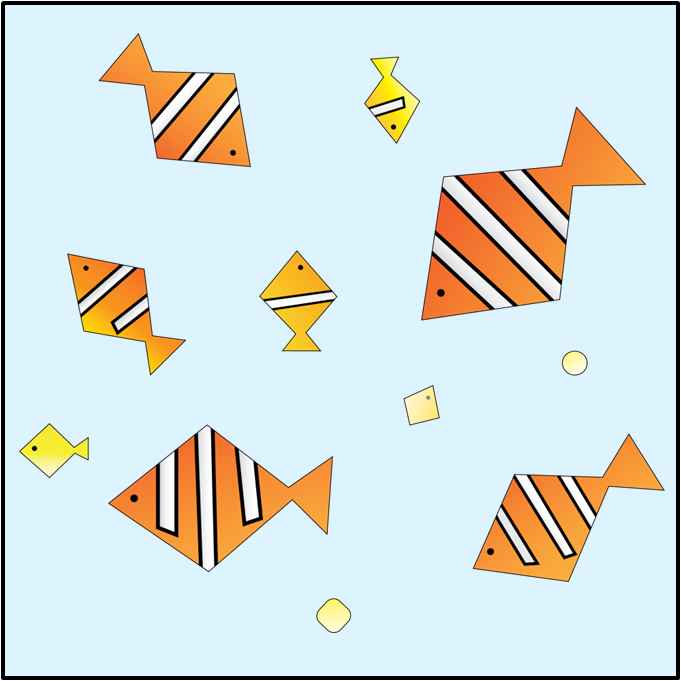
\includegraphics[width=\textwidth]{fish1}
\caption{}
\end{subfigure}
\begin{subfigure}{0.25\textwidth}
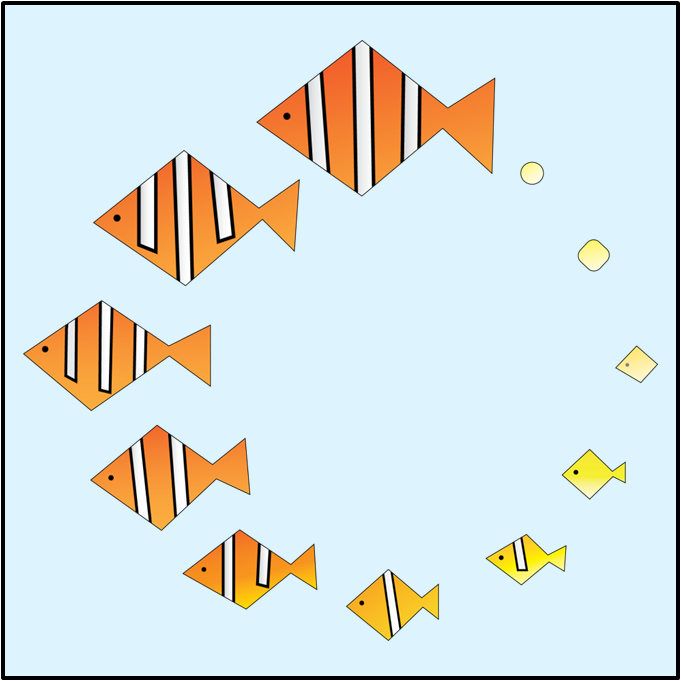
\includegraphics[width=\textwidth]{fish2}
\caption{}
\end{subfigure}
\caption{Schematic illustration of reconstructing dynamics from cross-sectional data. (a) Fish, each in a different orientation and a different stage of development. (b) Fish, now registered and temporally ordered. This is easy to do by hand because the data set is small and the developmental changes are easy to recognize.} 
\label{fig:fish}
\end{figure}

\begin{figure}
\begin{subfigure}{0.25\textwidth}
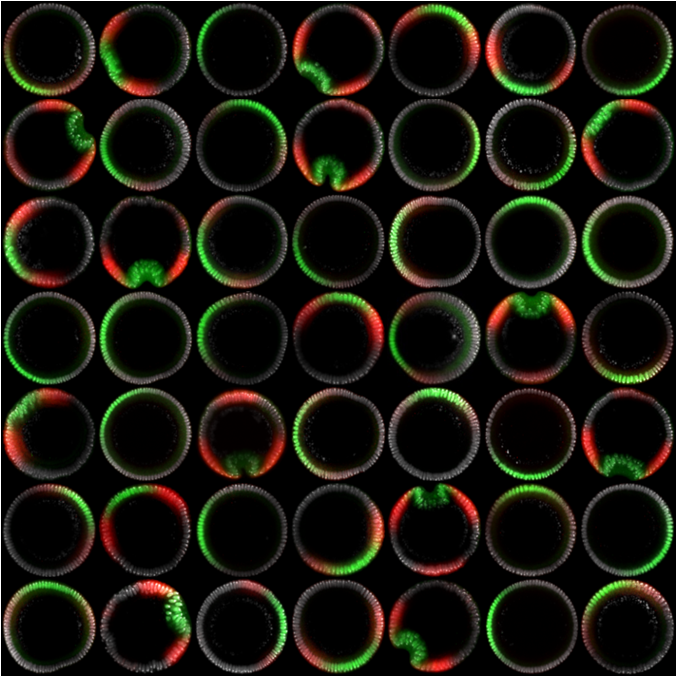
\includegraphics[width=\textwidth]{fig2a}
\caption{}
\label{subfig:images_scrambled}
\end{subfigure}
\begin{subfigure}{0.25\textwidth}
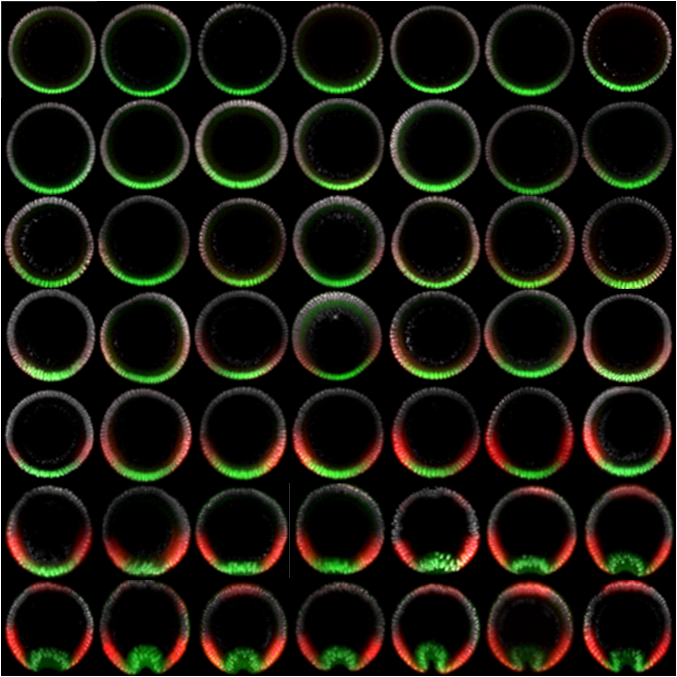
\includegraphics[width=\textwidth]{fig2b}
\caption{}
\label{subfig:images_hand_ordered}
\end{subfigure}
\caption{{\em Drosophila} data. (a) Dorsal-ventral images of {\em Drosphila} embryos in nuclear cycle 14, each stained for Dorsal (green) and dpERK (red). (b) Images from (a), now registered using the location of the Dorsal peak, and temporally ordered using the membrane marker.} 
\label{fig:fluorescent_images}
\end{figure}

\begin{figure*}
\begin{subfigure}{0.17\textwidth}

\includegraphics[width=\textwidth]{illustrate_1d}
\caption{}
\label{subfig:1d_image_example}
\end{subfigure}
\begin{subfigure}{0.2\textwidth}
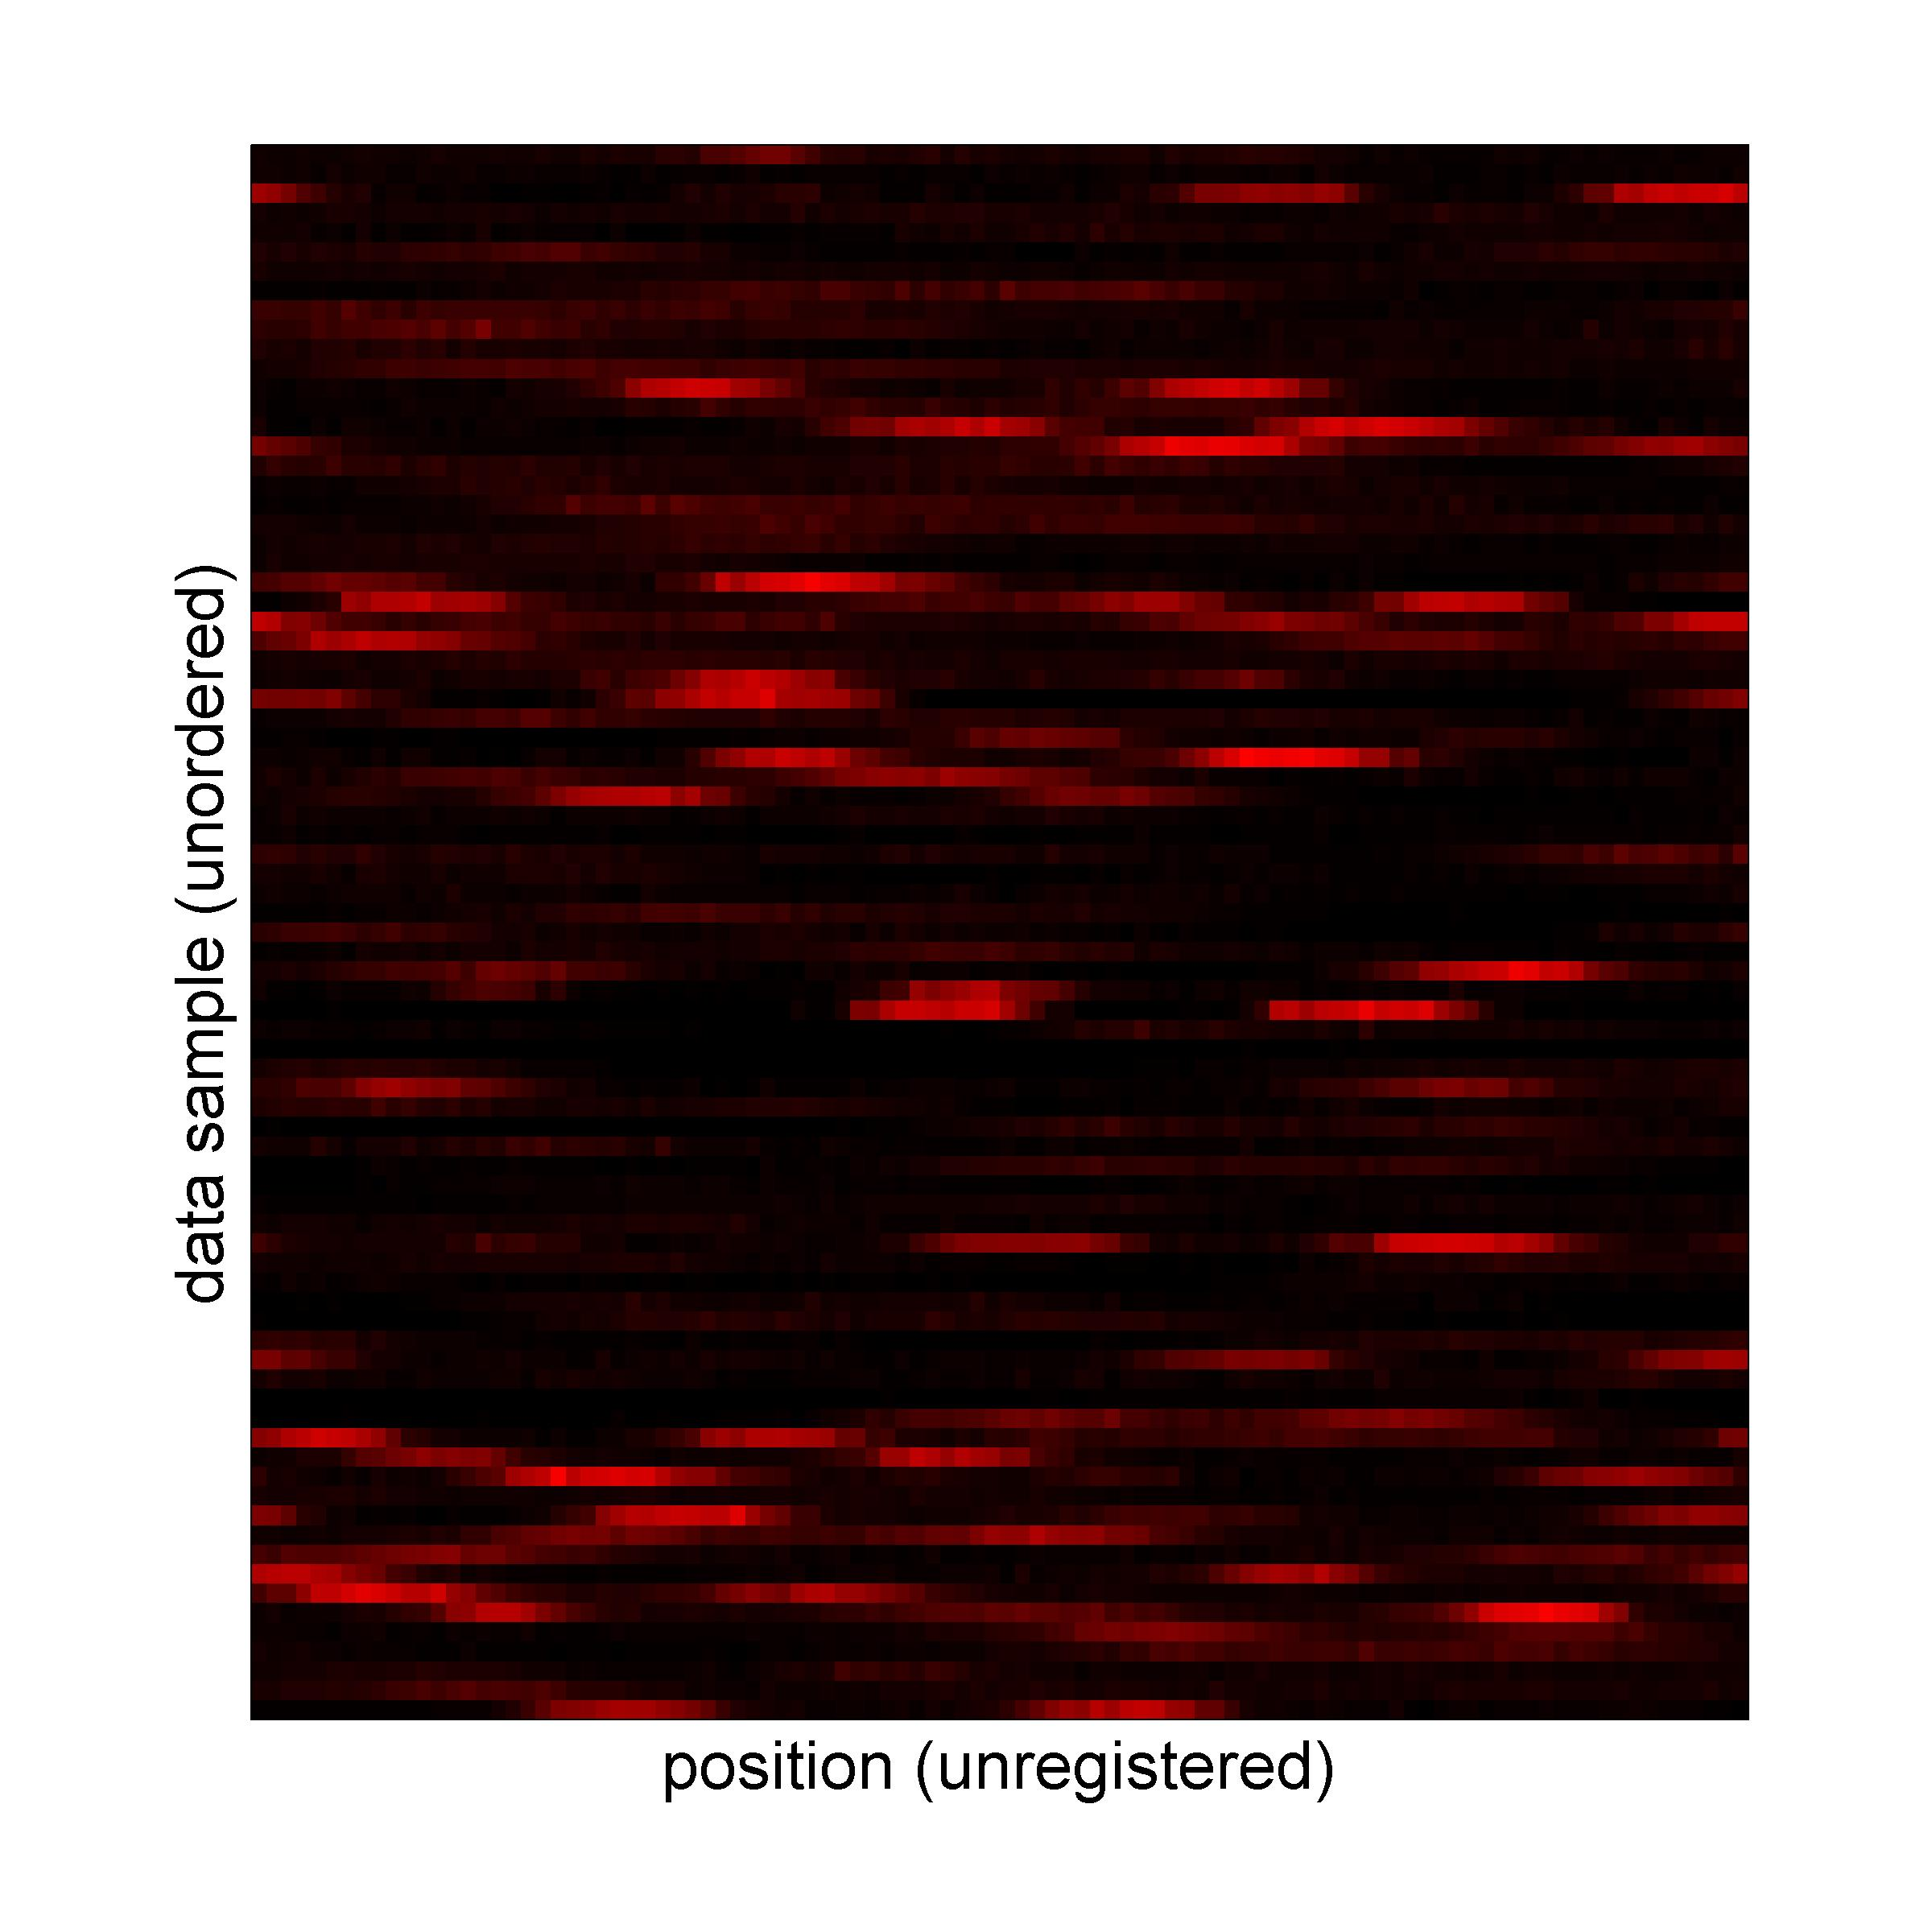
\includegraphics[width=\textwidth]{unregistered_unordered_1d}
\caption{}
\label{subfig:1d_unaligned_unordered}
\end{subfigure}
\begin{subfigure}{0.2\textwidth}
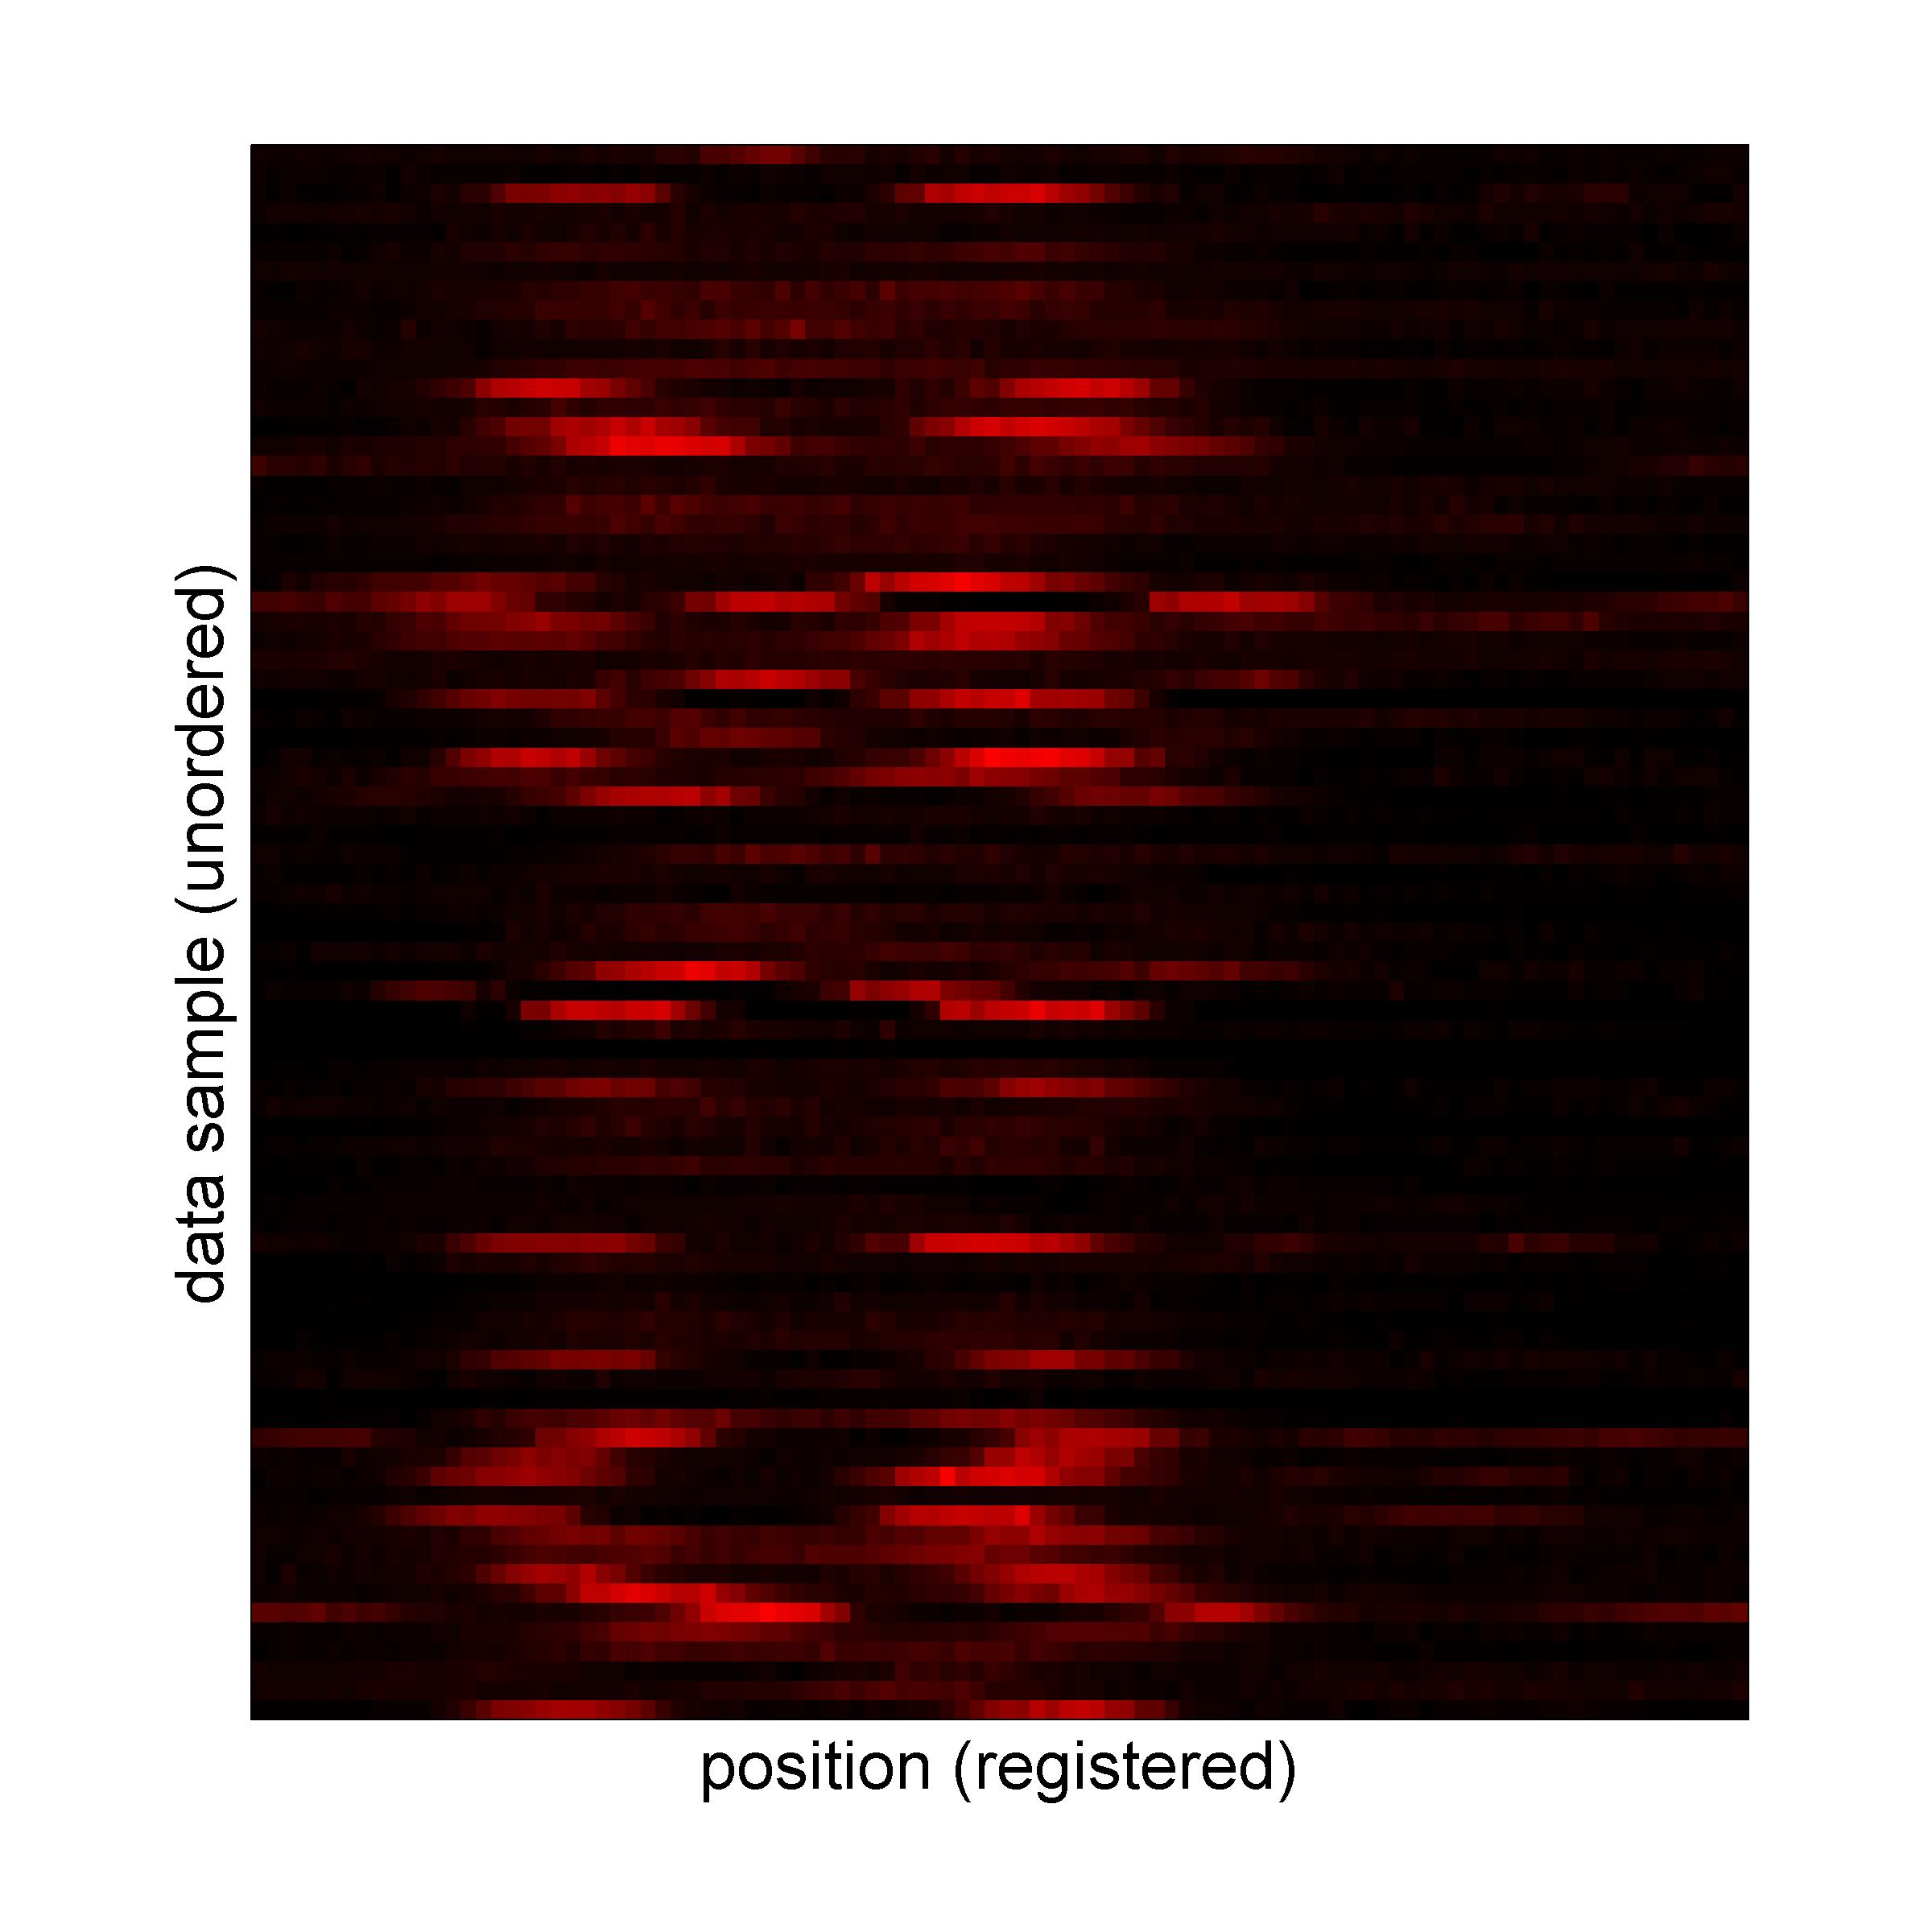
\includegraphics[width=\textwidth]{registered_unordered_1d}
\caption{}
\label{subfig:1d_aligned_unordered}
\end{subfigure}
\begin{subfigure}{0.2\textwidth}
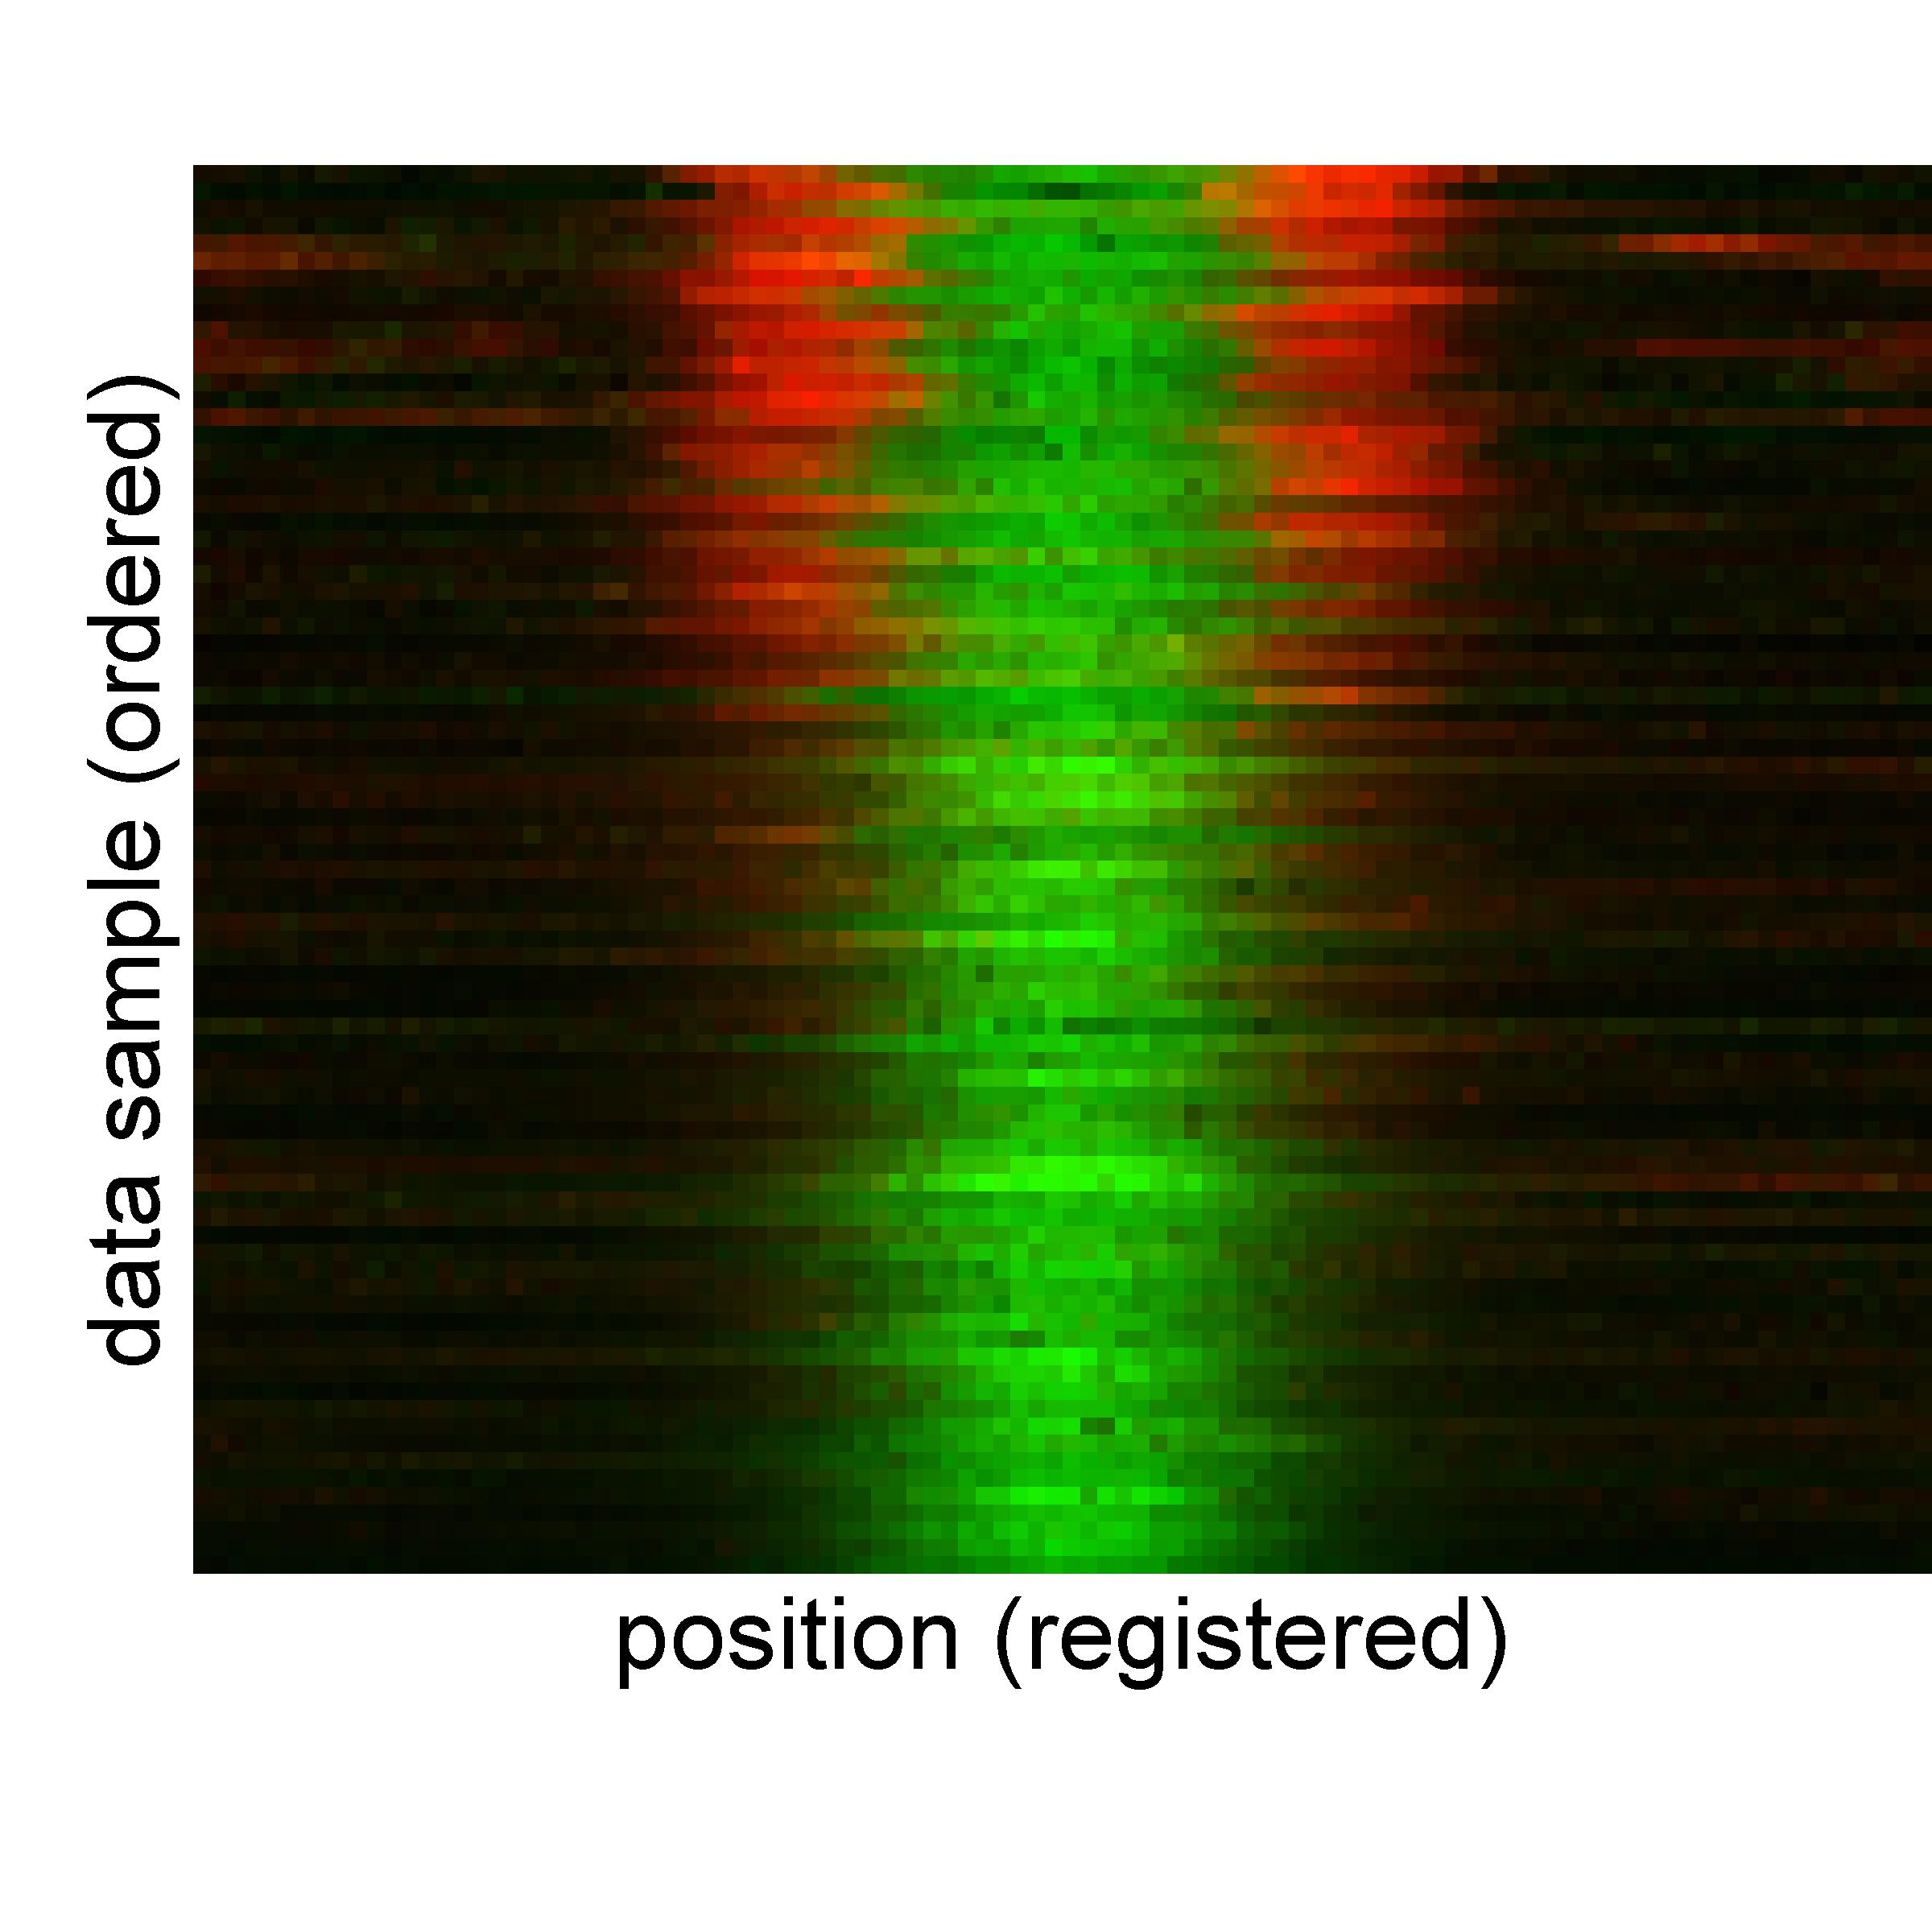
\includegraphics[width=\textwidth]{registered_ordered_1d}
\caption{}
\label{subfig:1d_aligned_ordered}
\end{subfigure}
\begin{subfigure}{0.2\textwidth}
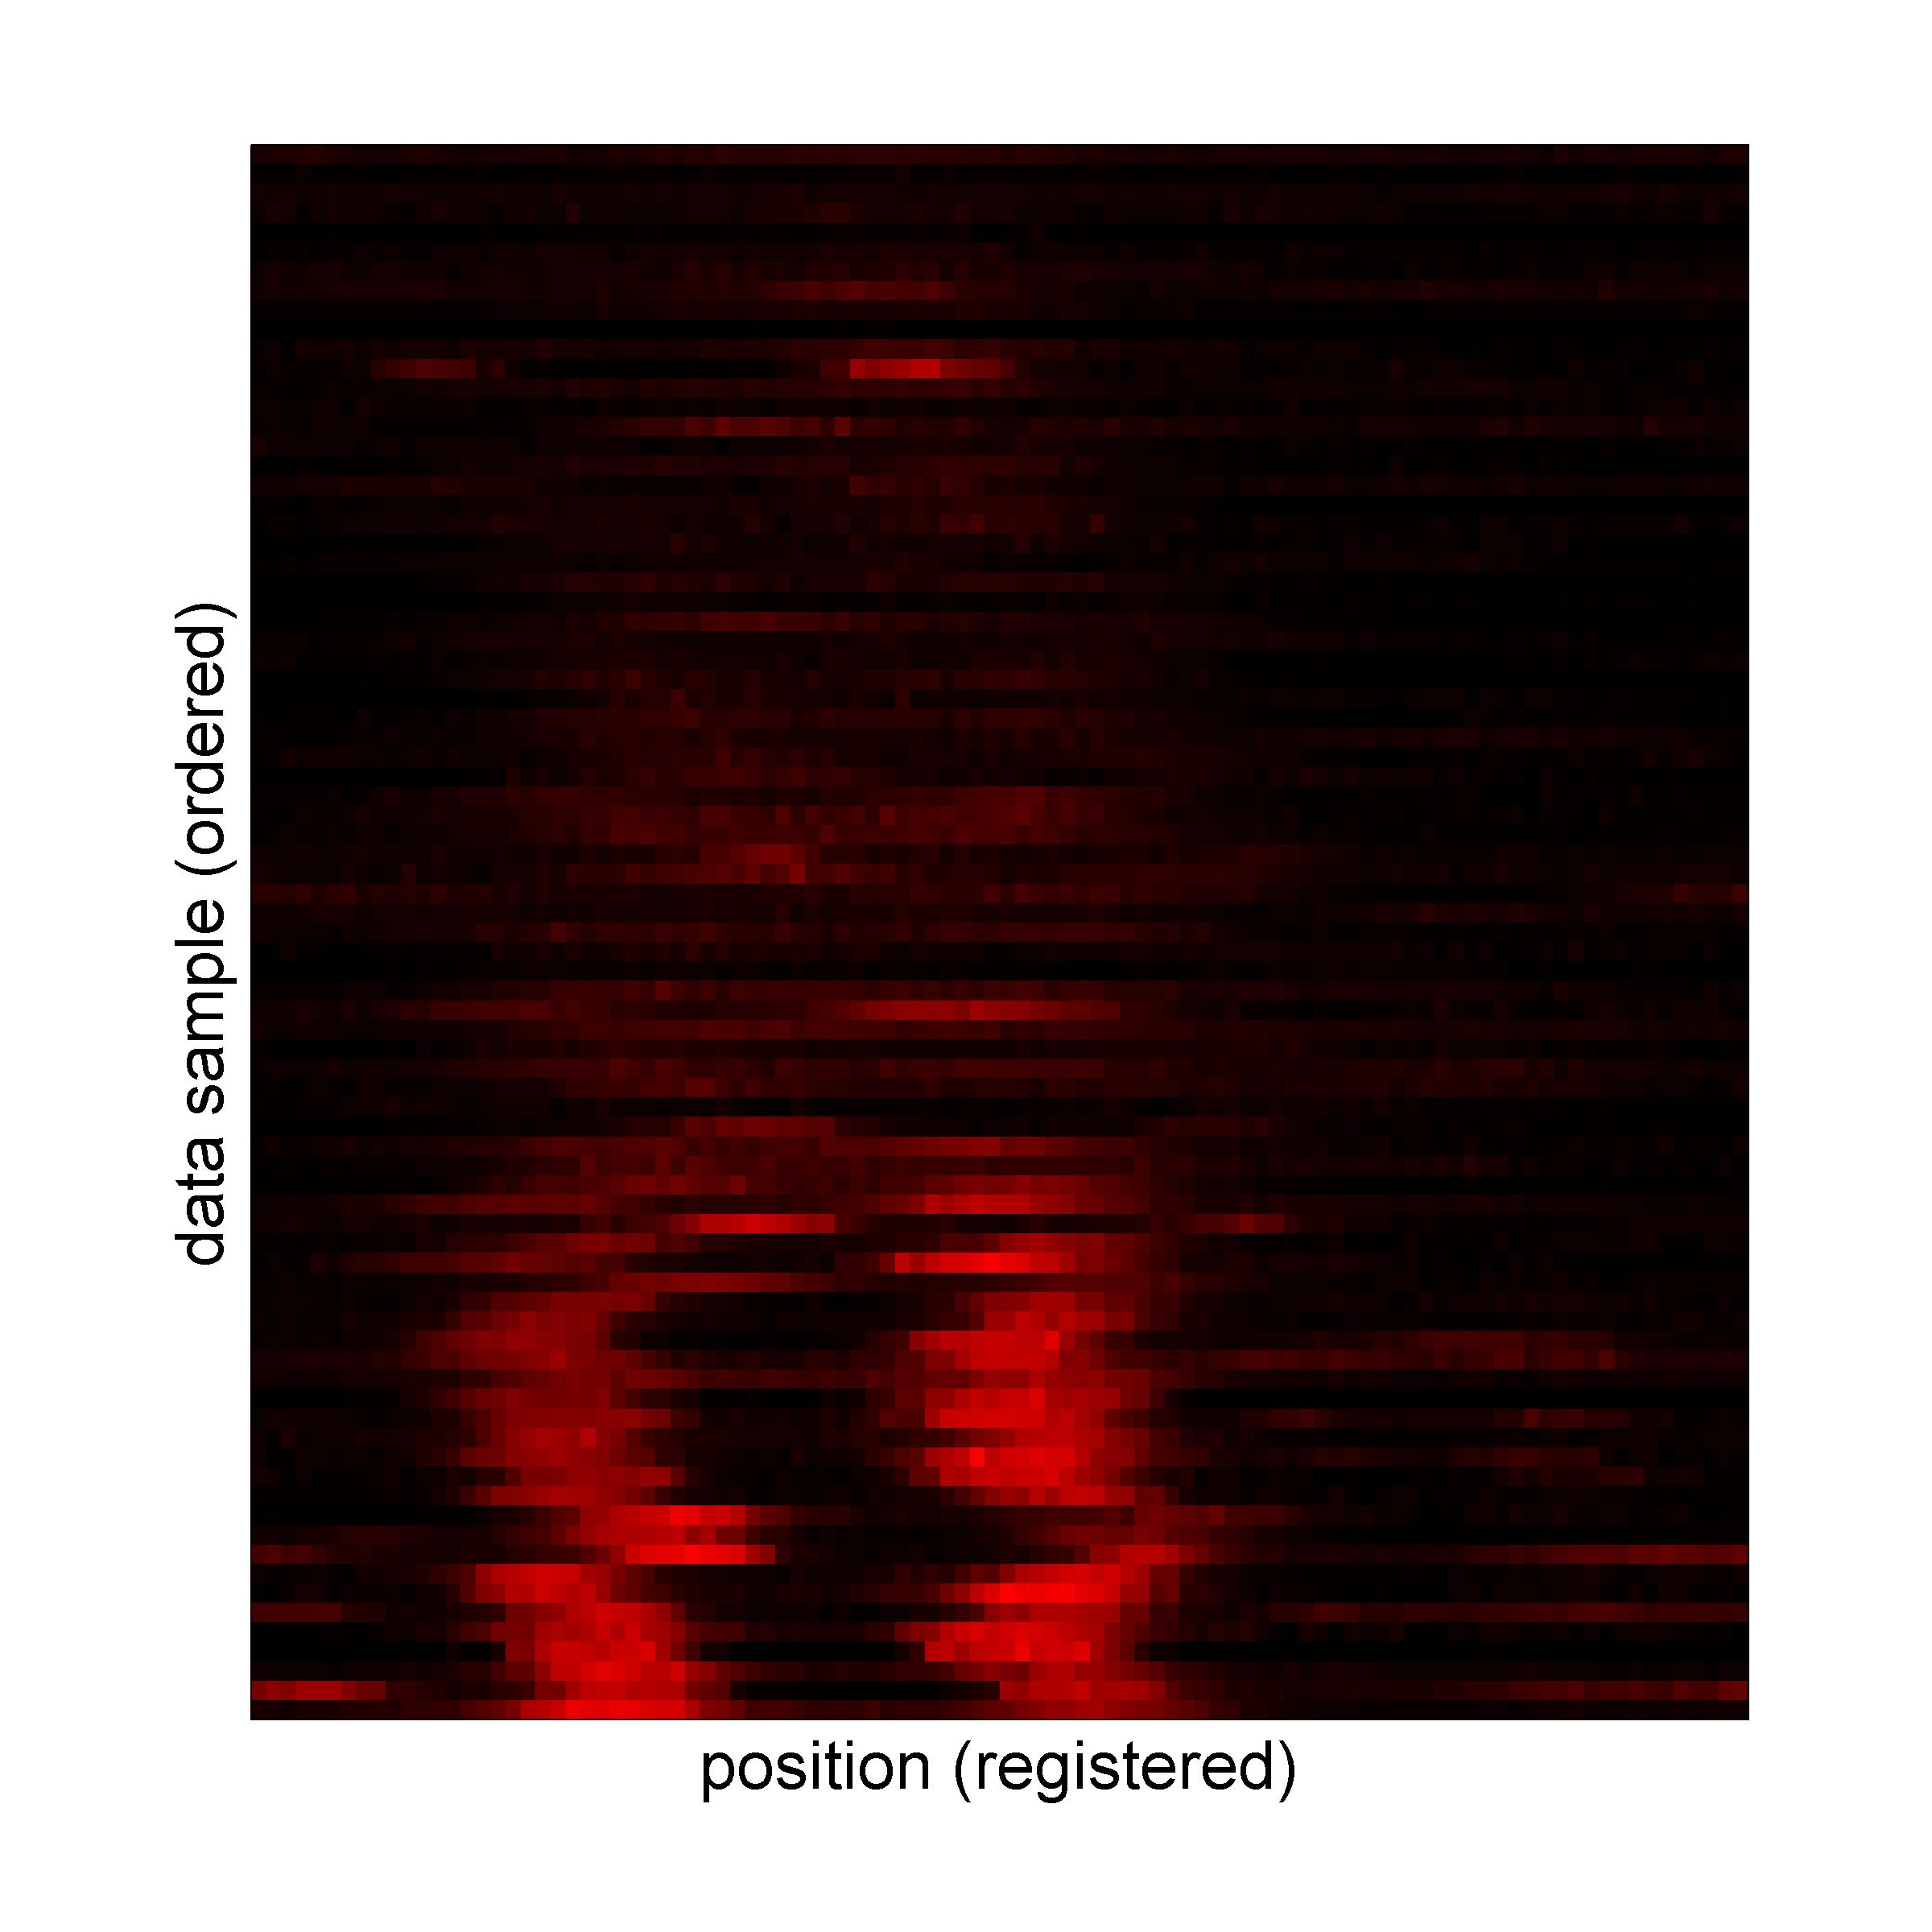
\includegraphics[width=\textwidth]{registered_ordered_vdm_1d}
\caption{}
\label{subfig:1d_aligned_ordered_vdm}
\end{subfigure}
\caption{(a) One-dimensional concentration profile on a ring (top), and the corresponding profile on a line (bottom). (b) The concentration profiles corresponding to the images in Figure \ref{fig:fluorescent_images}. Each row in the array corresponds to one image. (c) The concentration profiles in (b), now registered using angular synchronization. (d) The concentration profiles in (c), now temporally ordered using diffusion maps. (e) The concentration profiles in (b), now simultaneously registered and temporally ordered using vector diffusion maps. }
\label{fig:1d_demo}
\end{figure*}

\begin{figure*}
\begin{minipage}{0.6\textwidth}
\begin{subfigure}{\textwidth}
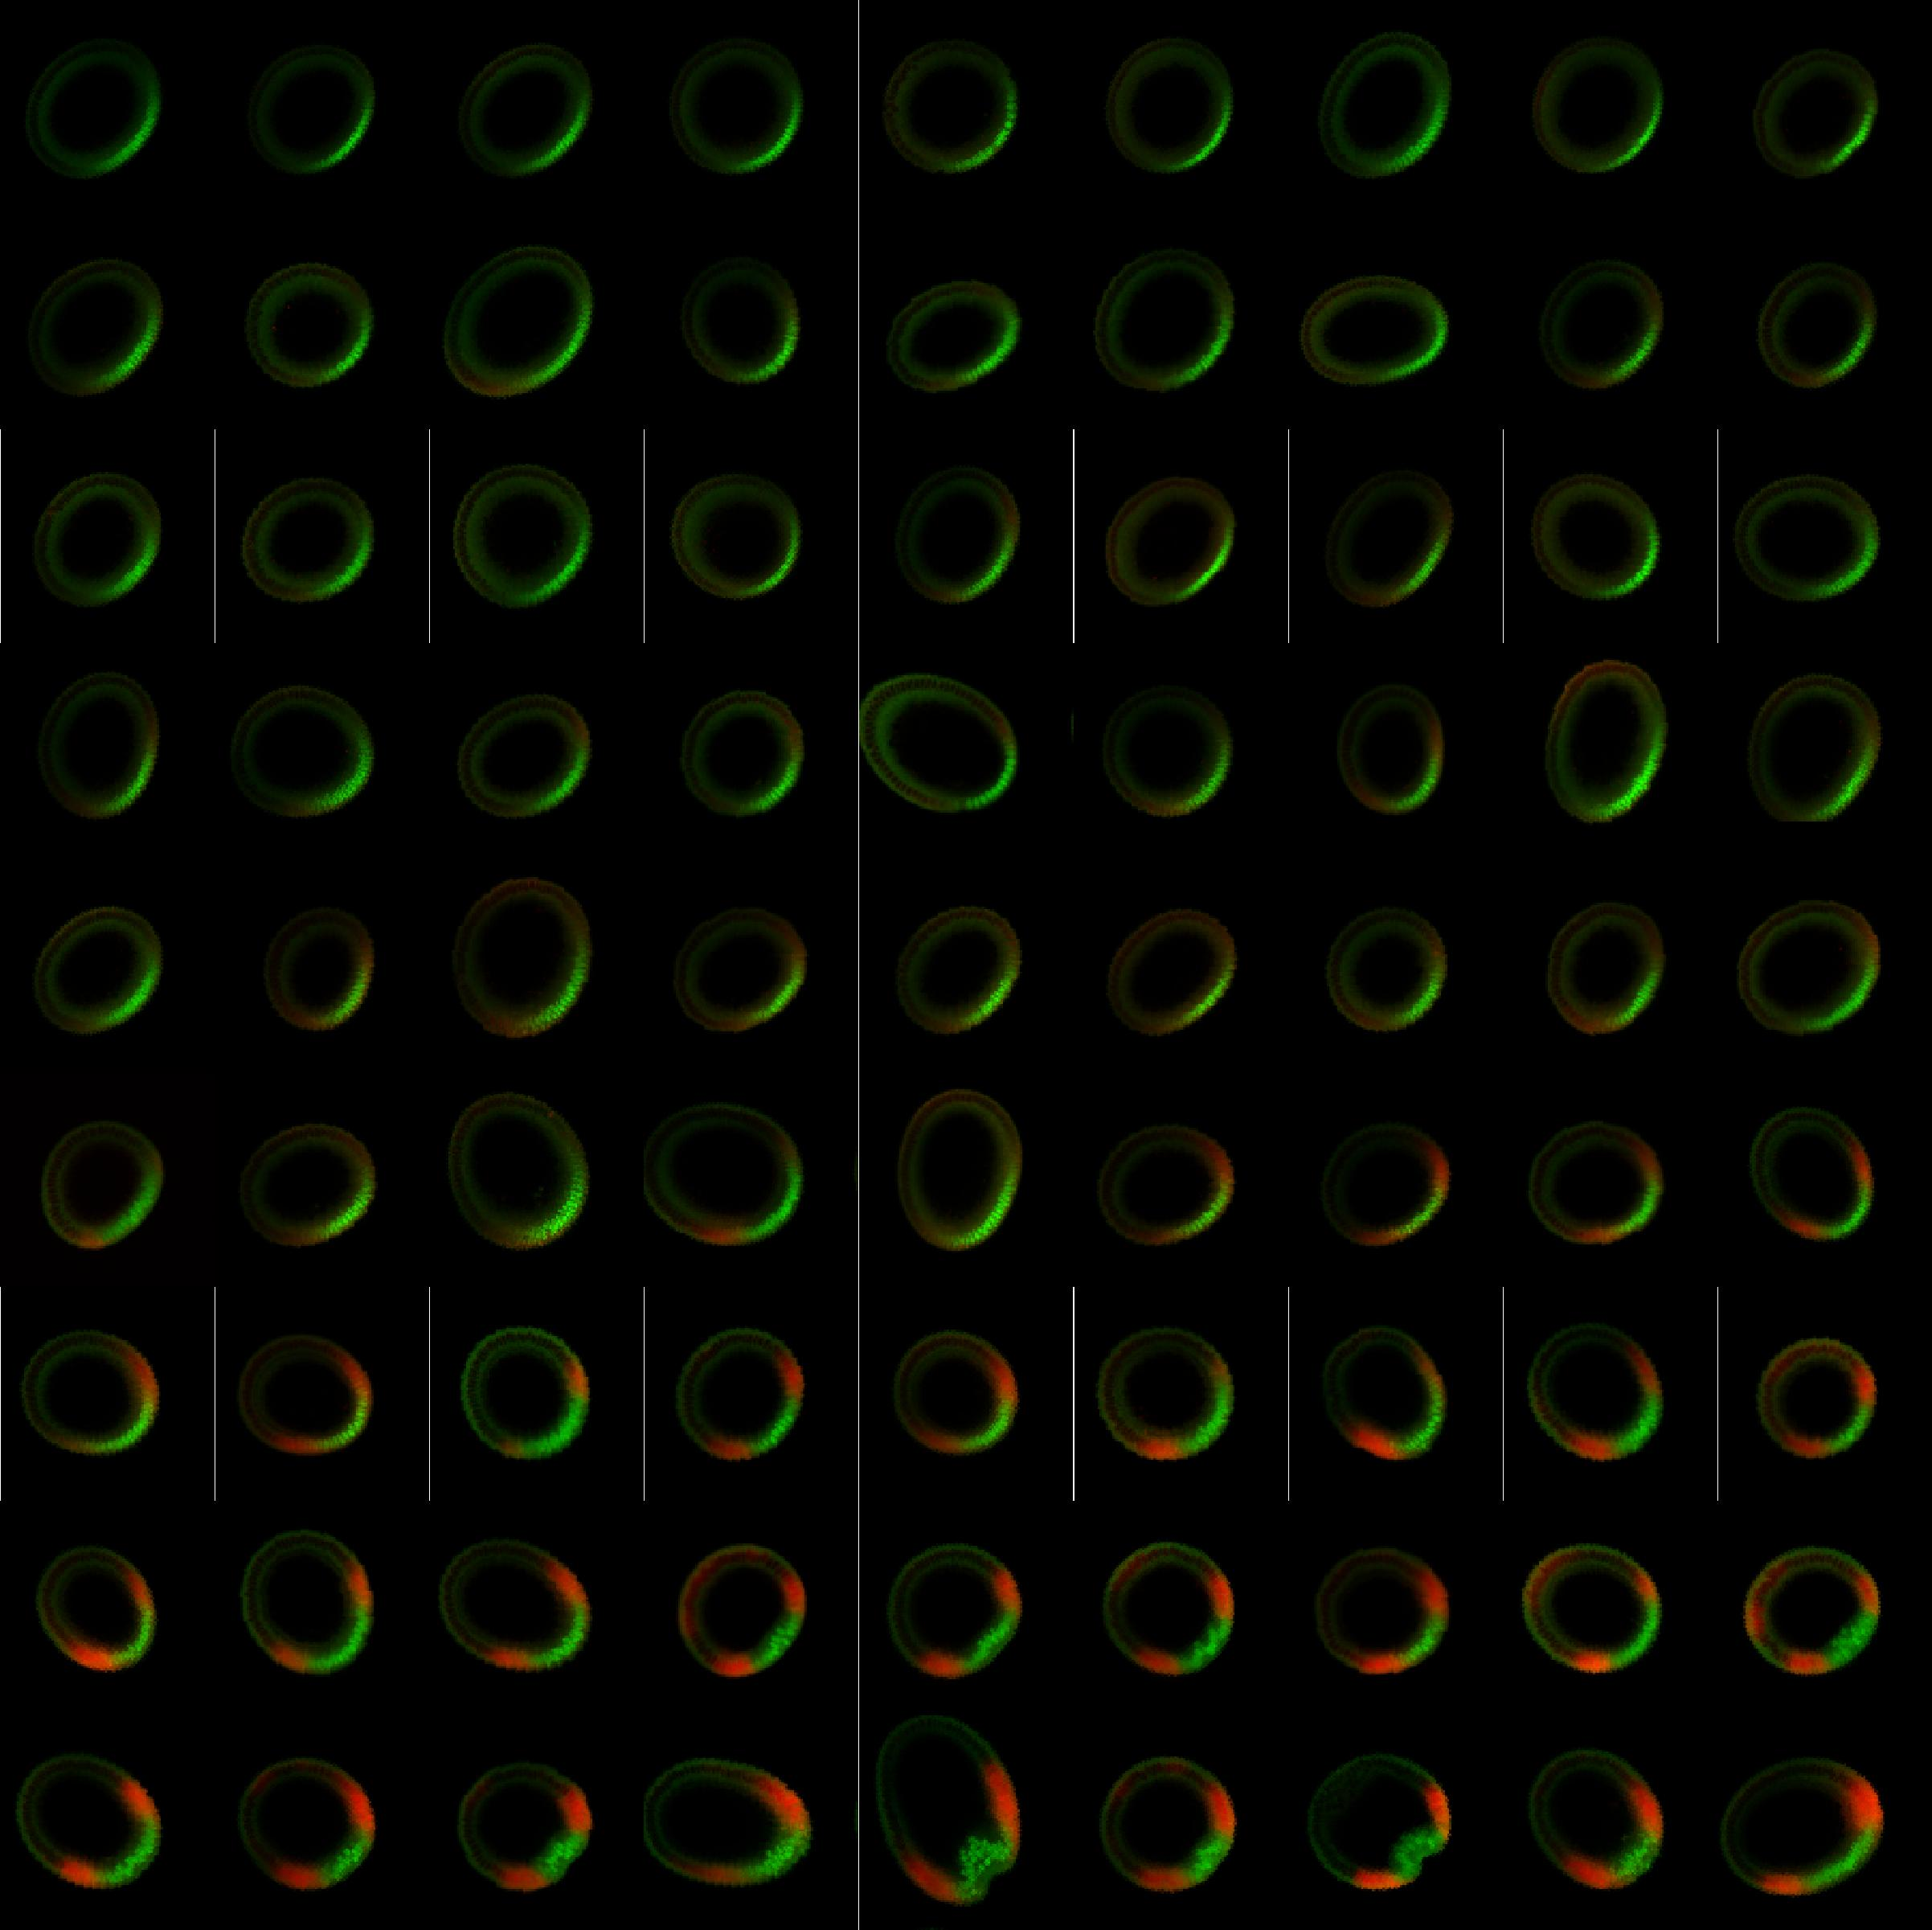
\includegraphics[width=\textwidth]{registered_ordered_vdm_2d}
\caption{}
\label{subfig:images_vdm}
\end{subfigure}
\end{minipage}
\begin{minipage}{0.4\textwidth}
\begin{subfigure}{\textwidth}
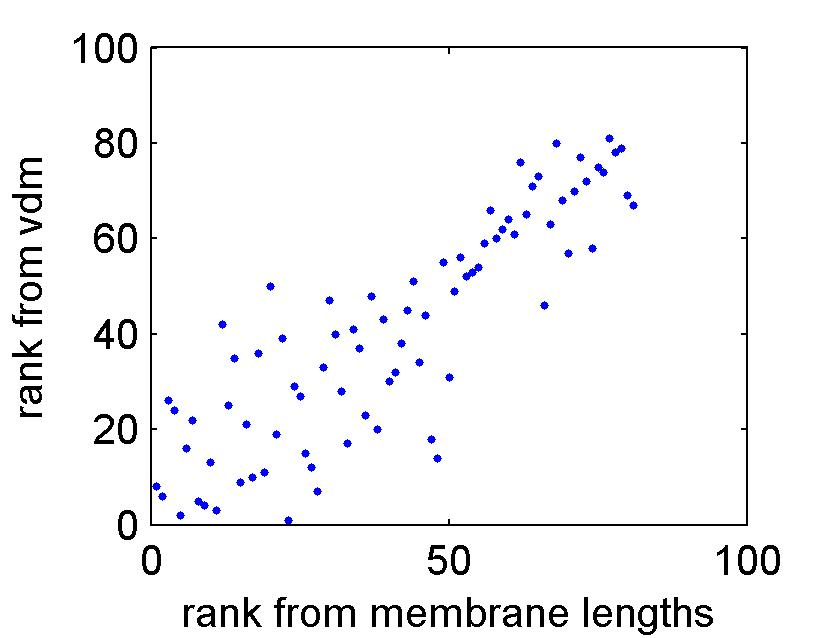
\includegraphics[width=\textwidth]{rank_corr_vdm}
\caption{}
\label{subfig:rank_corr}
\end{subfigure}
\begin{subfigure}{\textwidth}
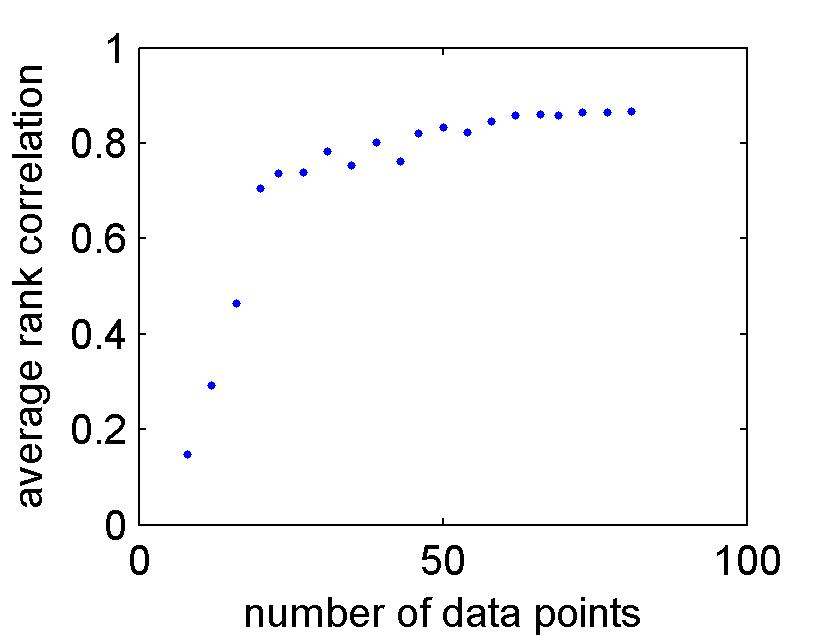
\includegraphics[width=\textwidth]{bootstrap_rank_corr_color}
\caption{}
\label{subfig:bootstrap}
\end{subfigure}
\end{minipage}
\caption{(a) The images in Figure~\ref{fig:fluorescent_images}, aligned and temporally ordered using vector diffusion maps. (b) The rank correlation between the ordering of the images in (a) using vector diffusion maps, and the ordering obtained using the membrane markers. (c) The rank correlation coefficient as a function of the number of data points. }
\end{figure*}

%\begin{figure*}
%\begin{subfigure}{0.2\textwidth}
%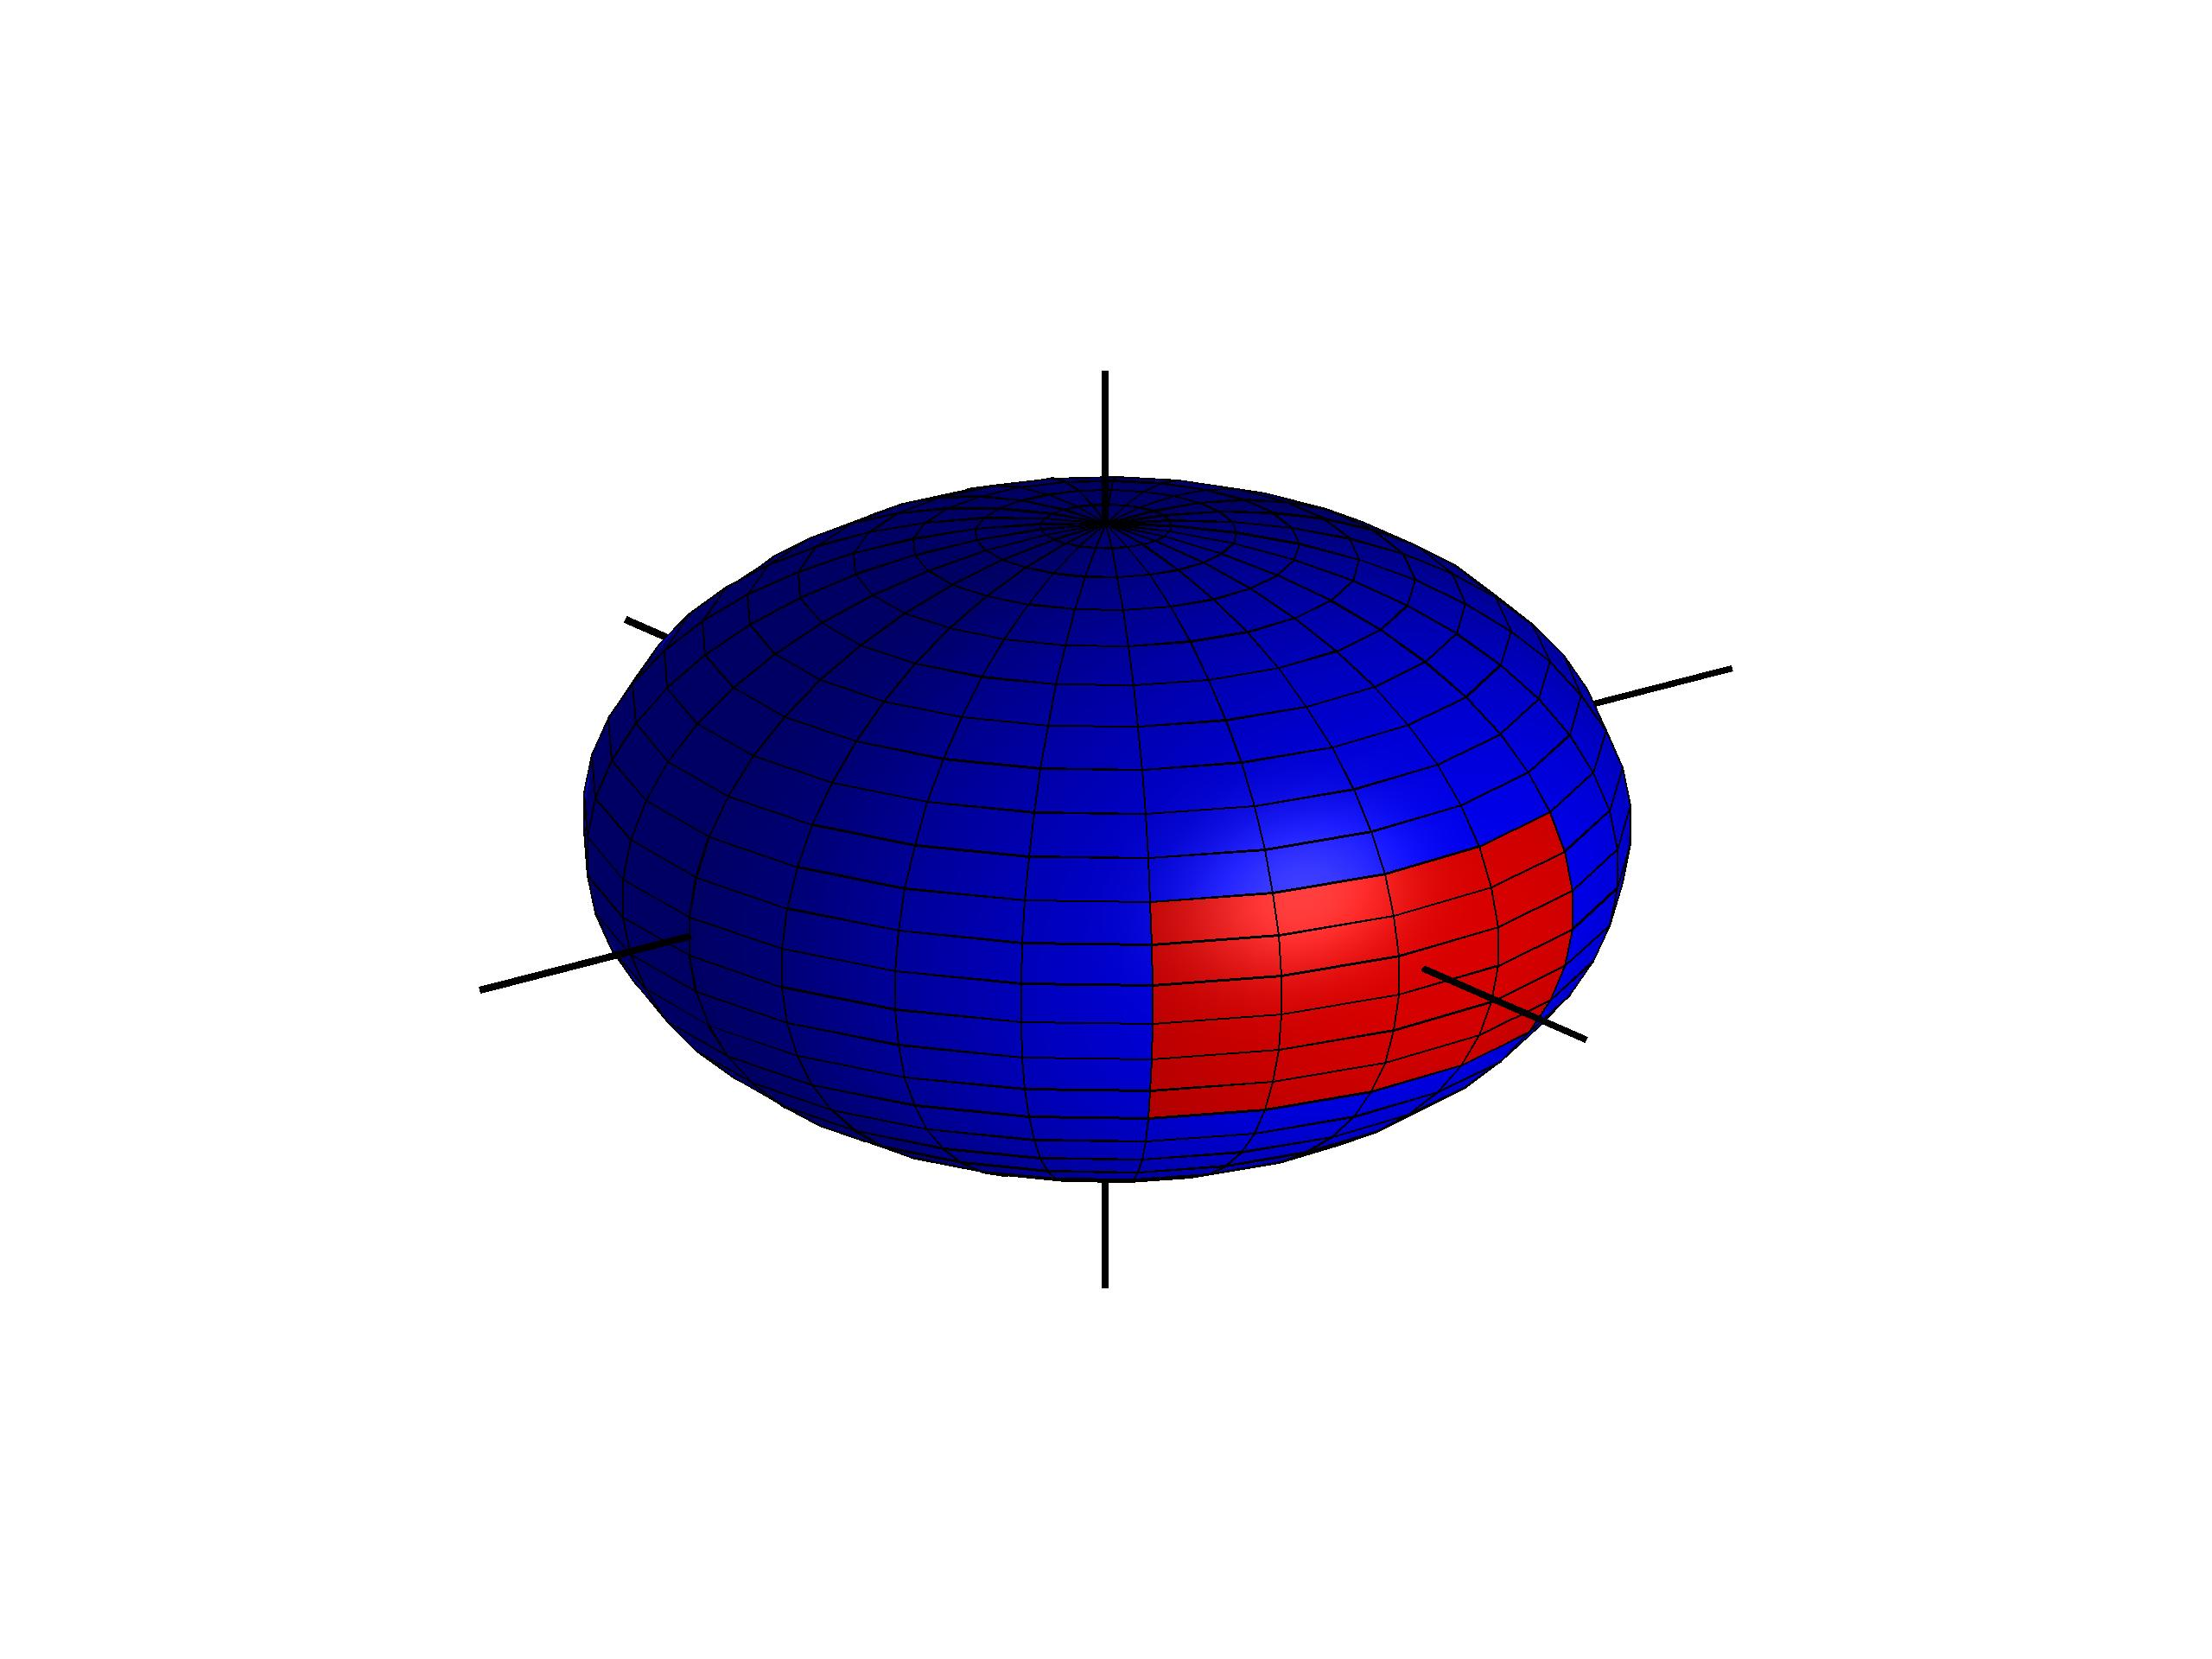
\includegraphics[width=\textwidth]{sphere_1}
%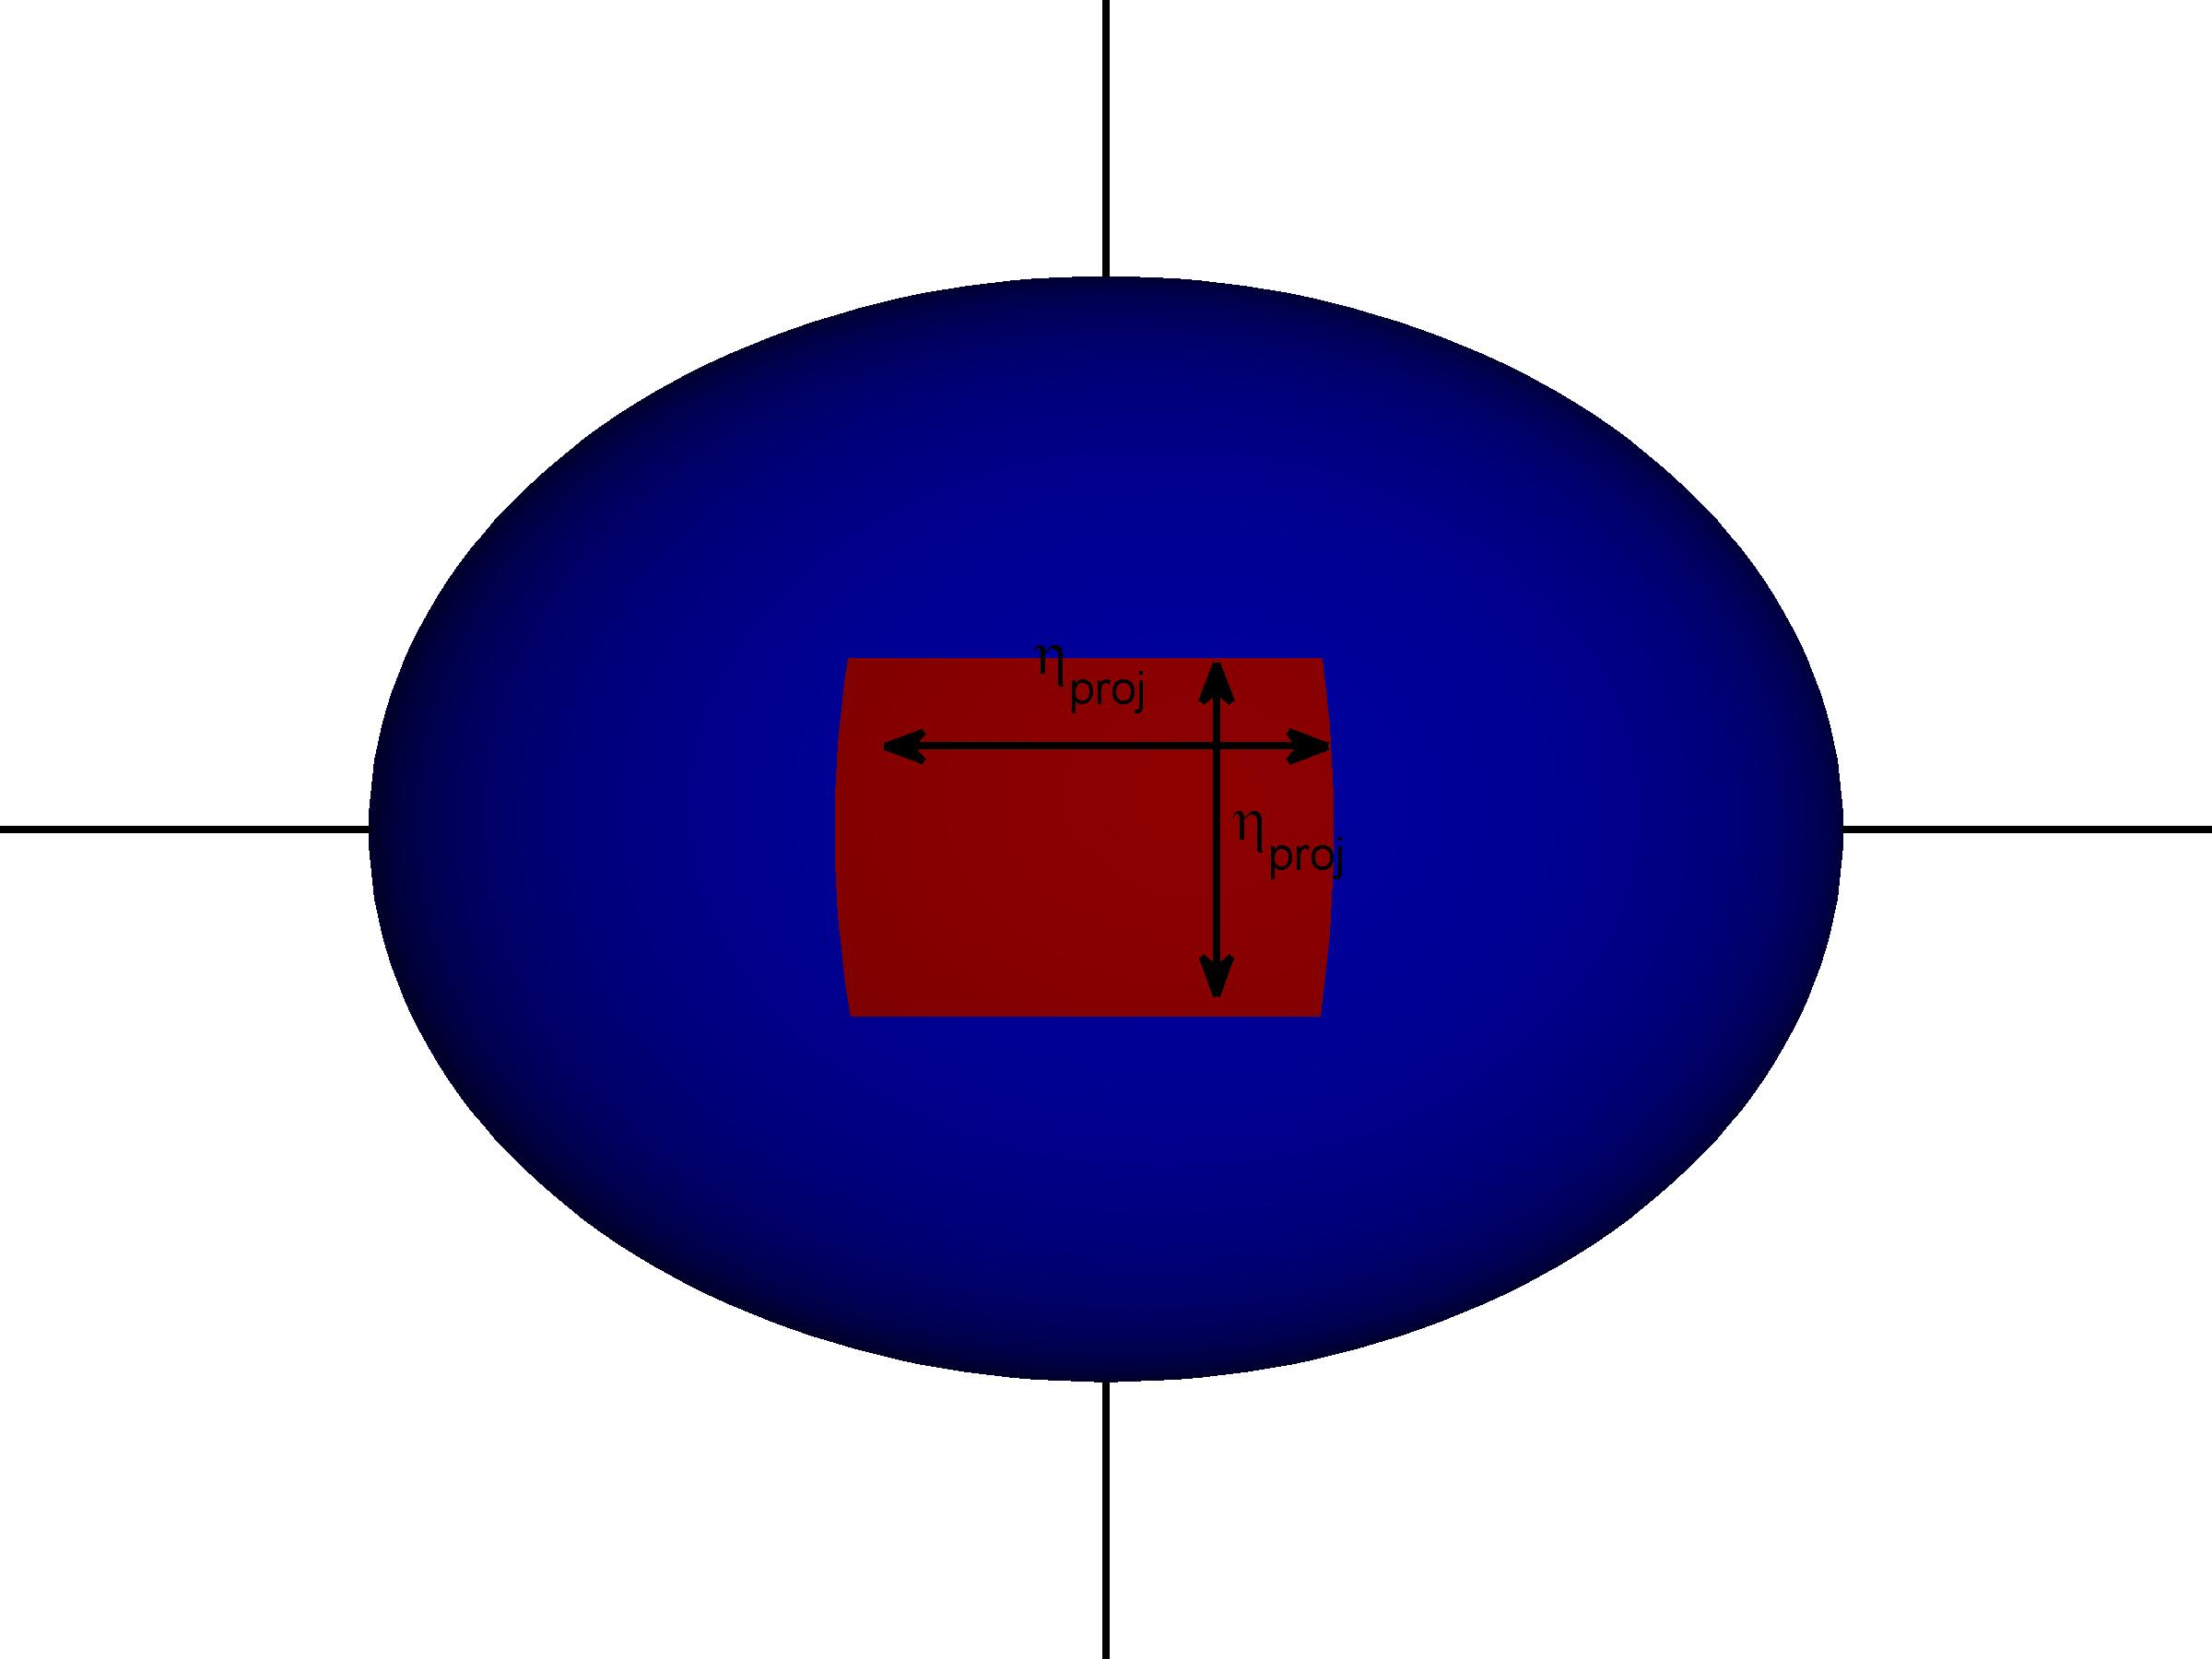
\includegraphics[width=\textwidth]{sphere2_1}
%\caption{}
%\end{subfigure}
%\begin{subfigure}{0.2\textwidth}
%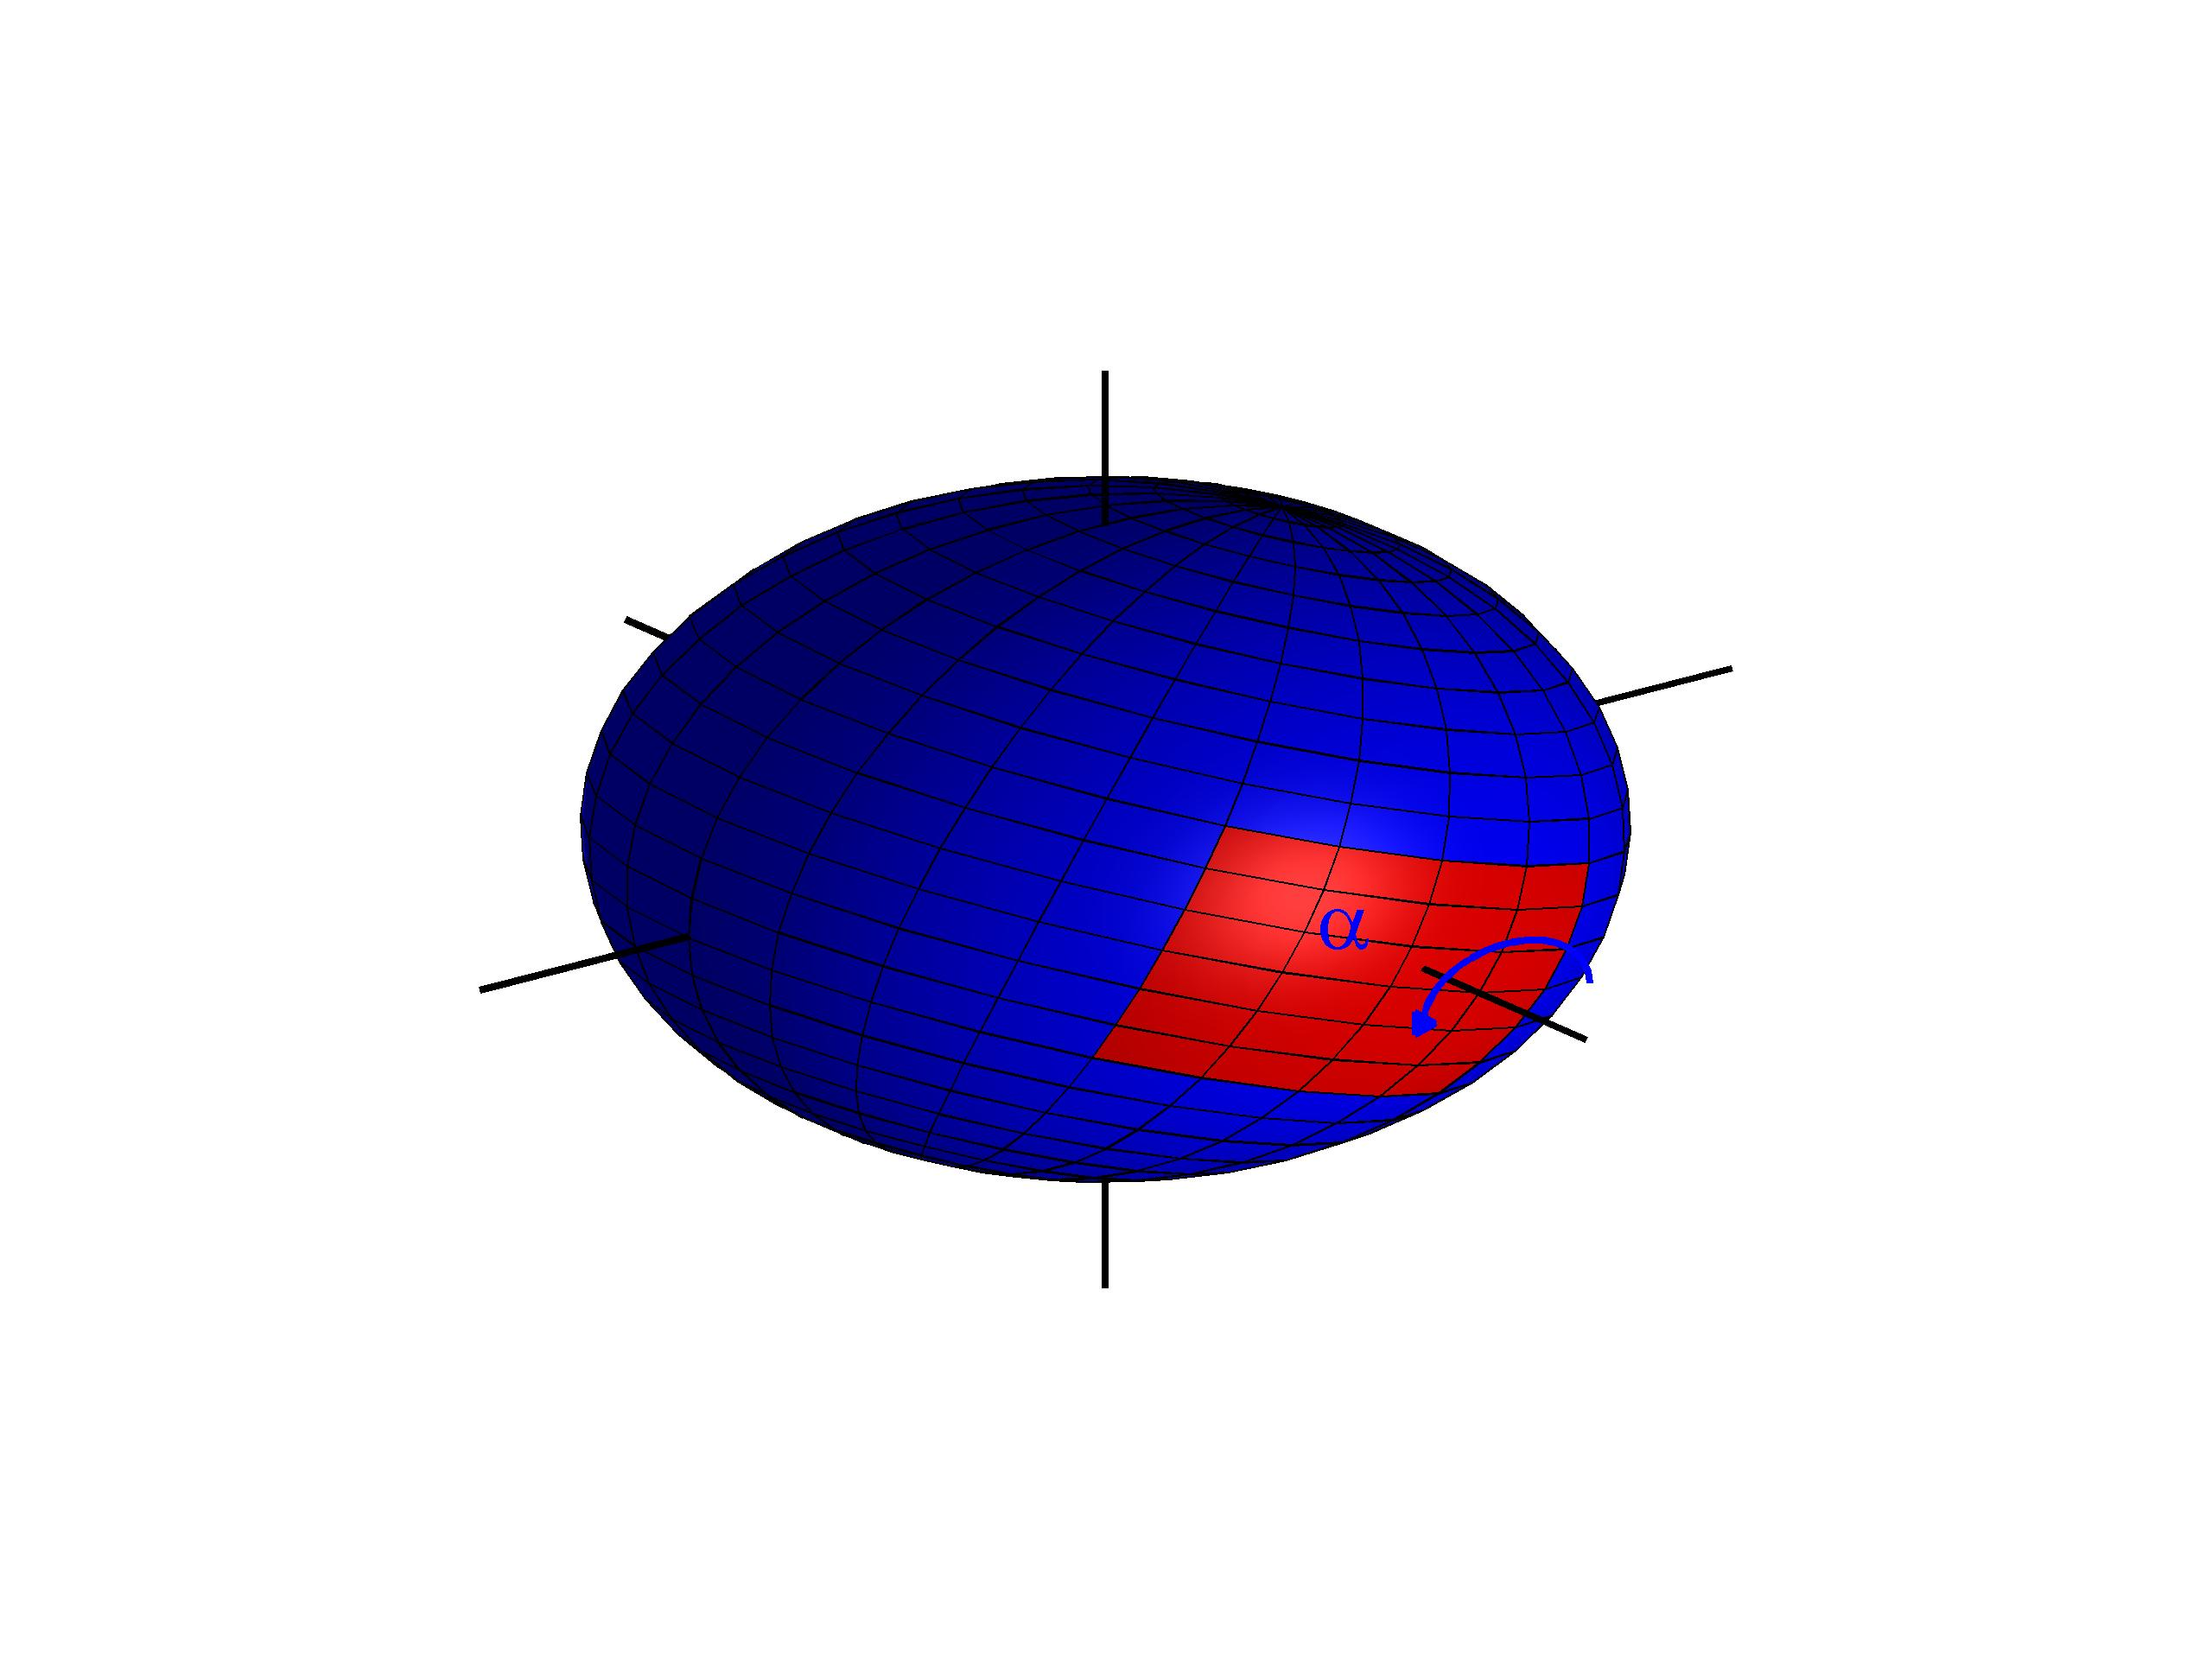
\includegraphics[width=\textwidth]{sphere_2}
%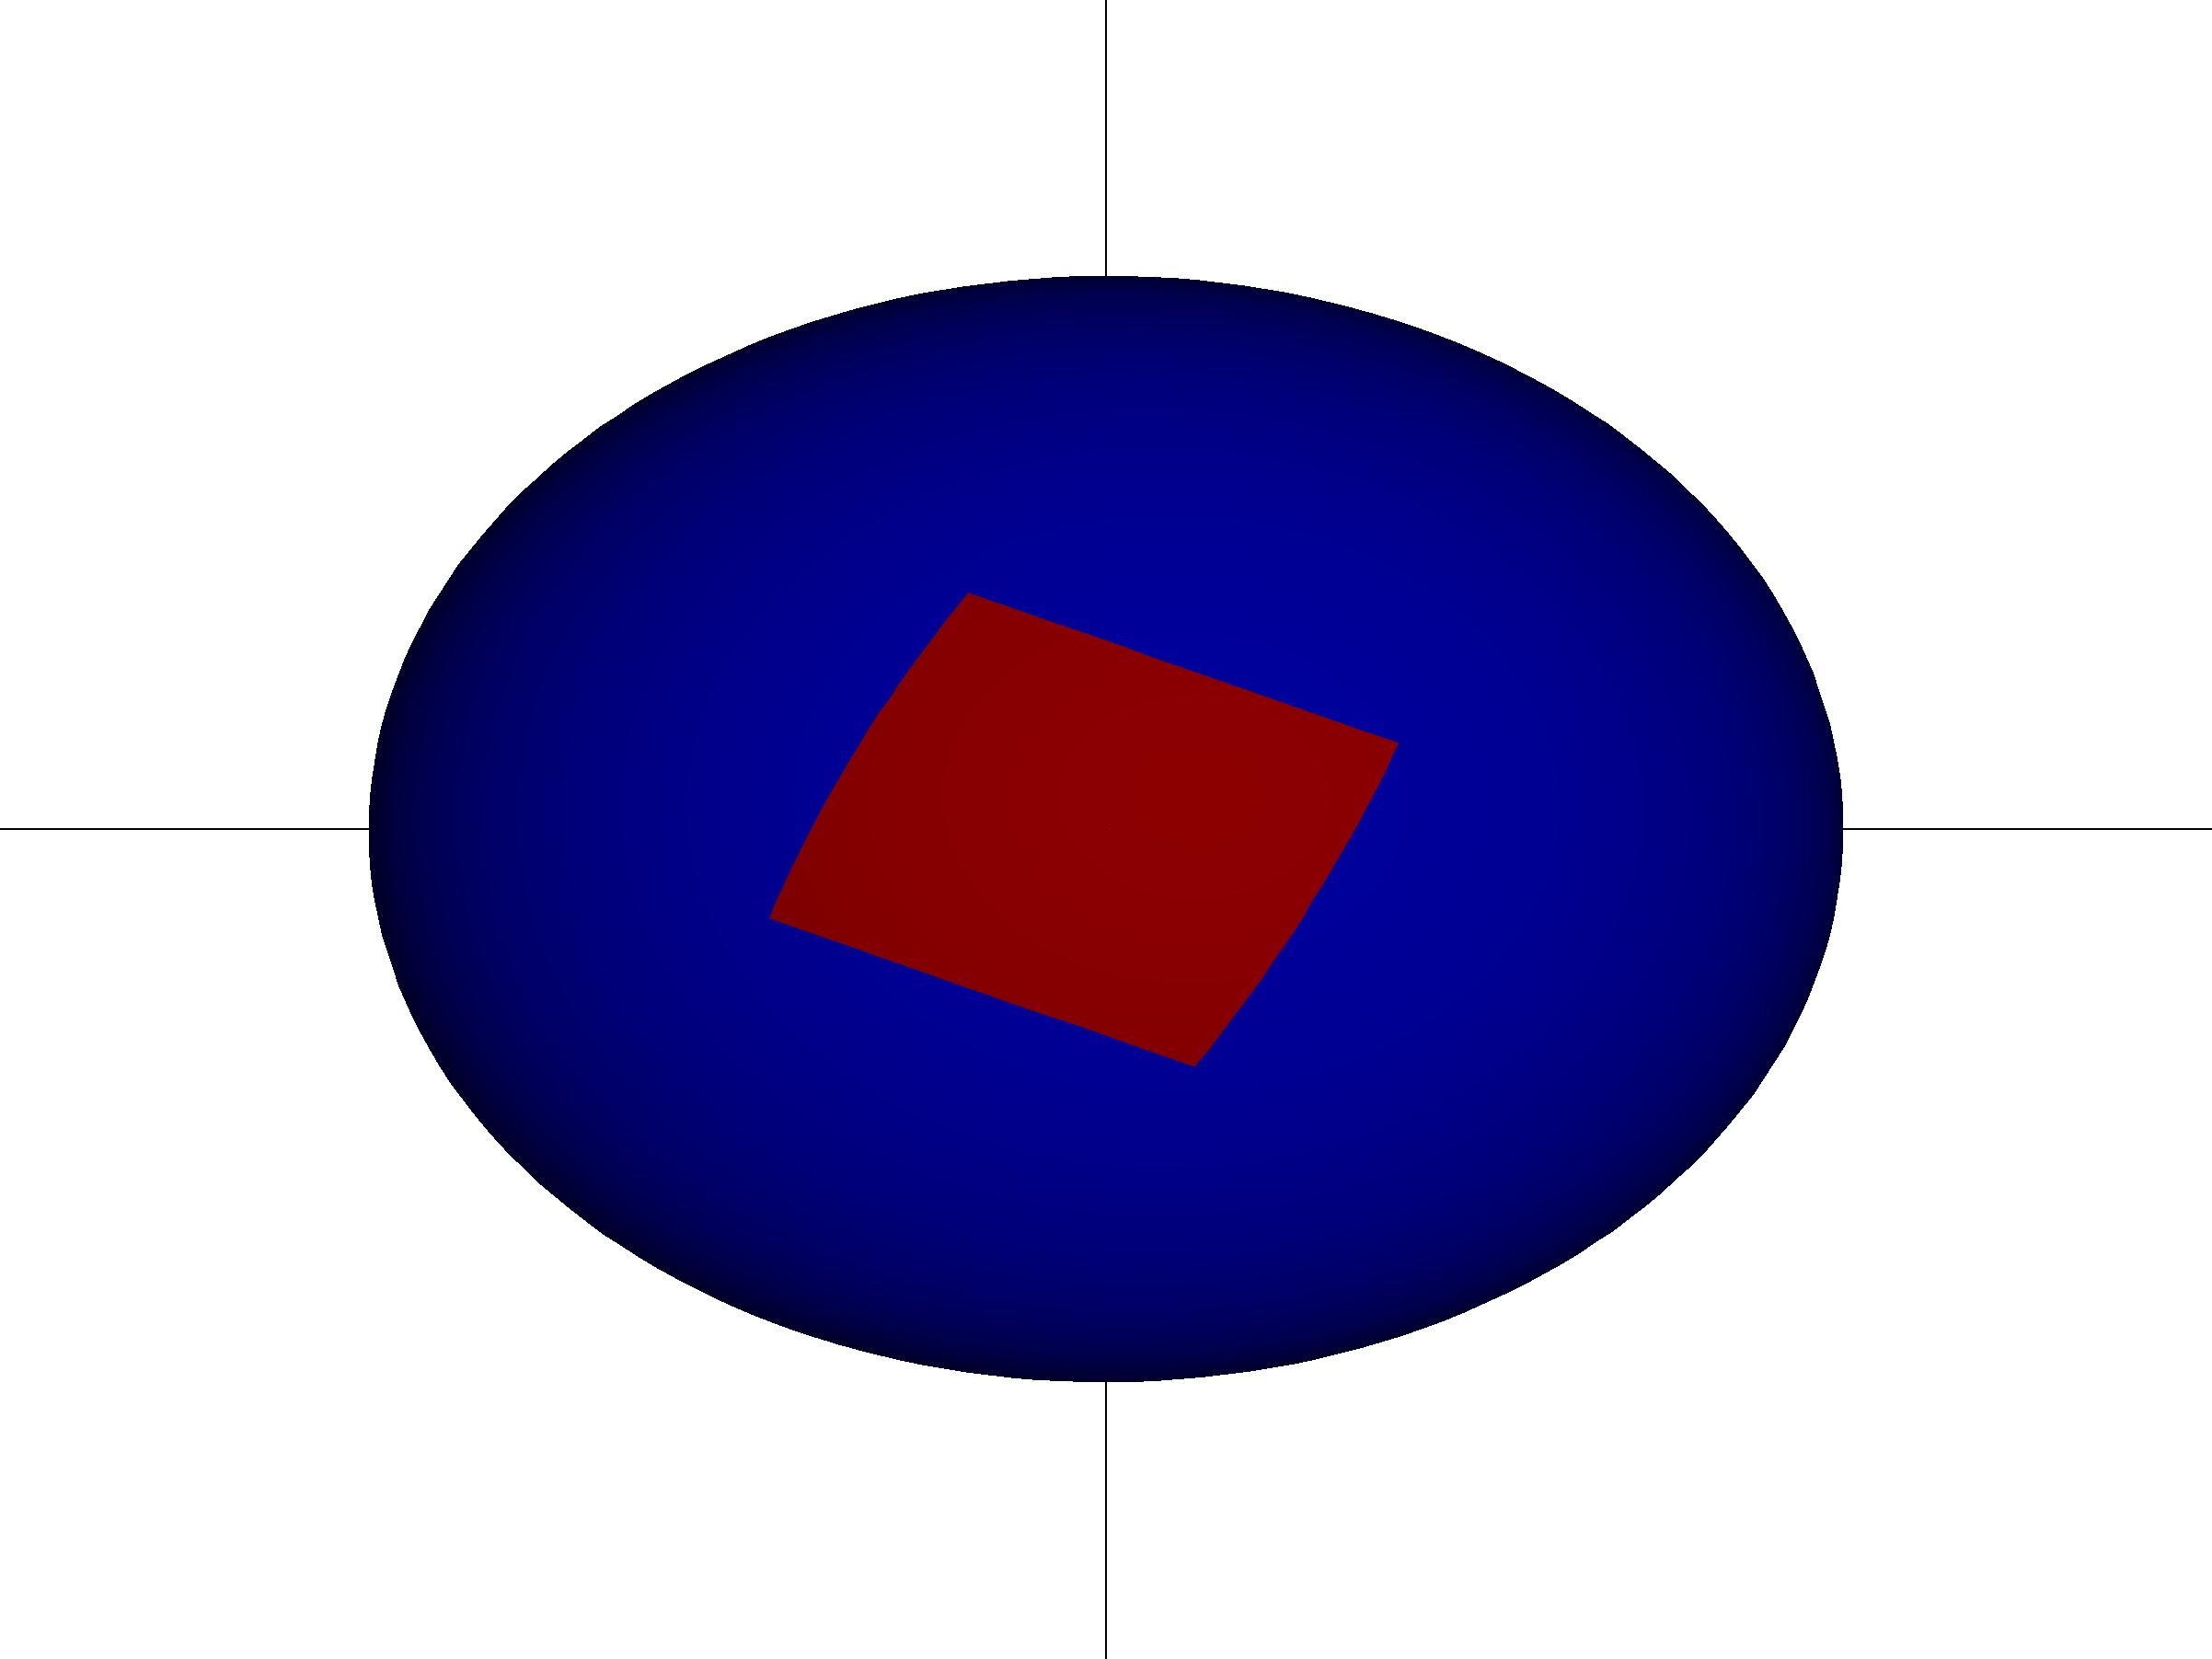
\includegraphics[width=\textwidth]{sphere2_2}
%\caption{}
%\end{subfigure}
%\begin{subfigure}{0.2\textwidth}
%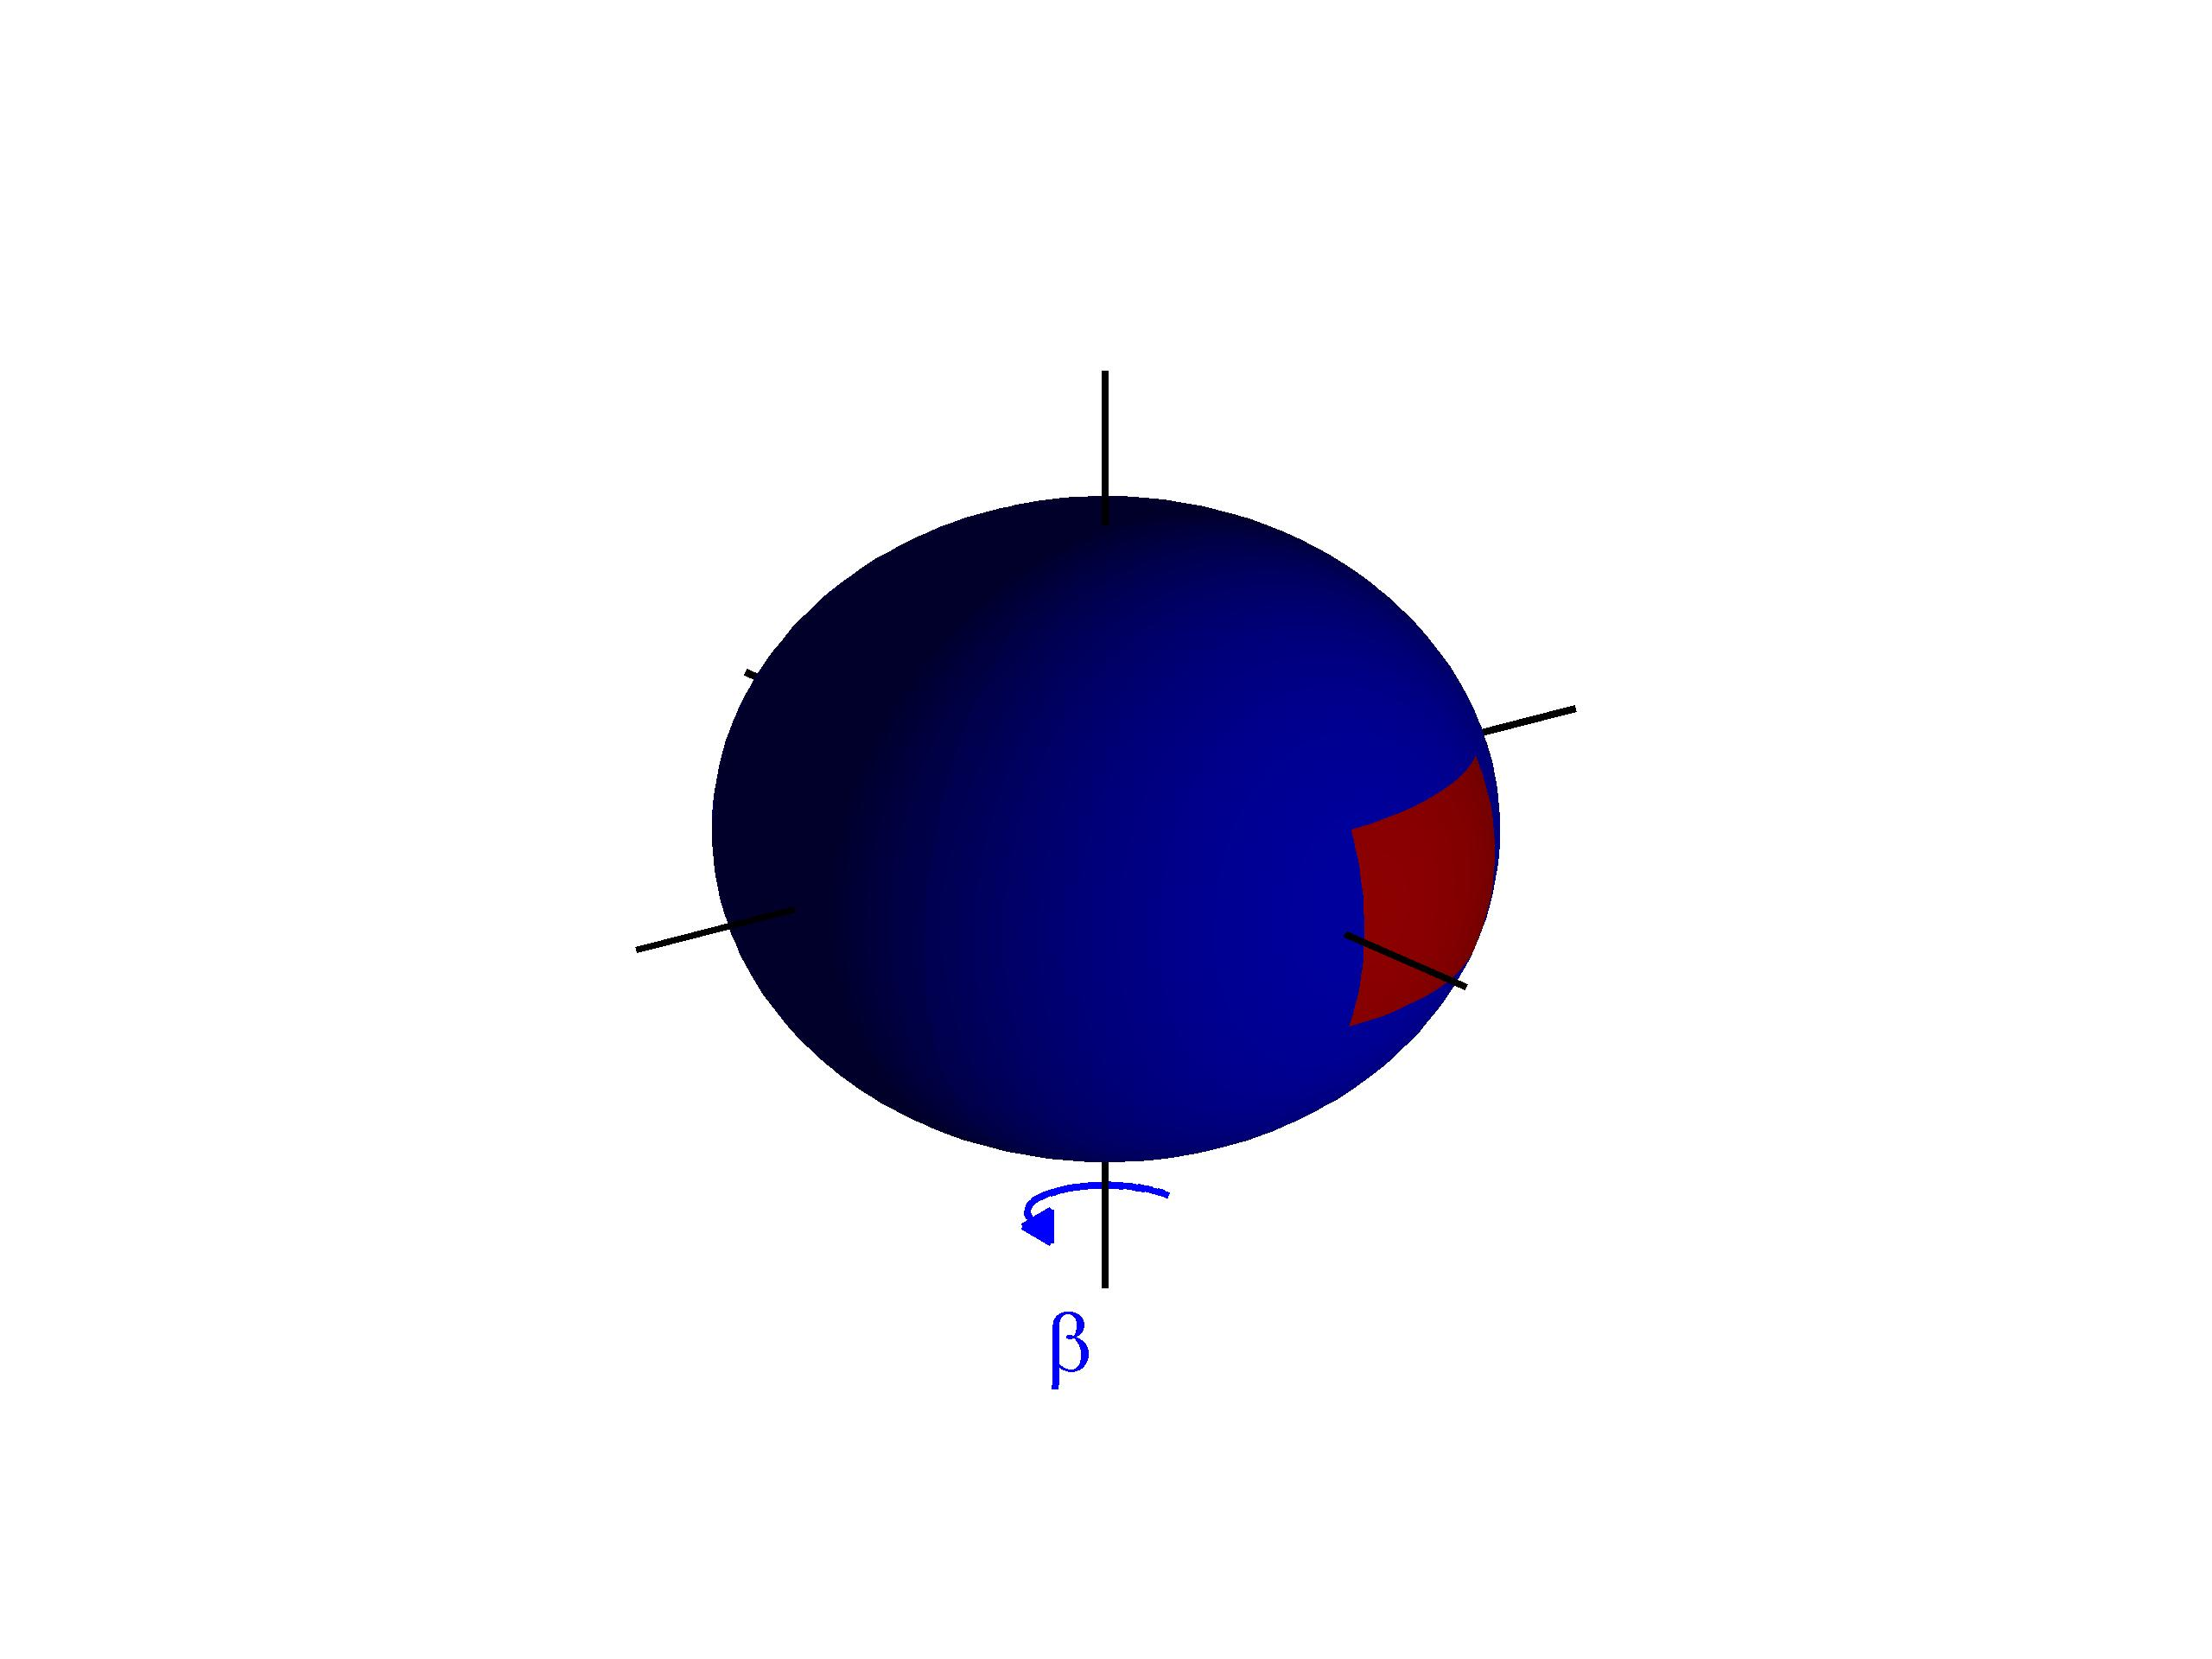
\includegraphics[width=\textwidth]{sphere_3}
%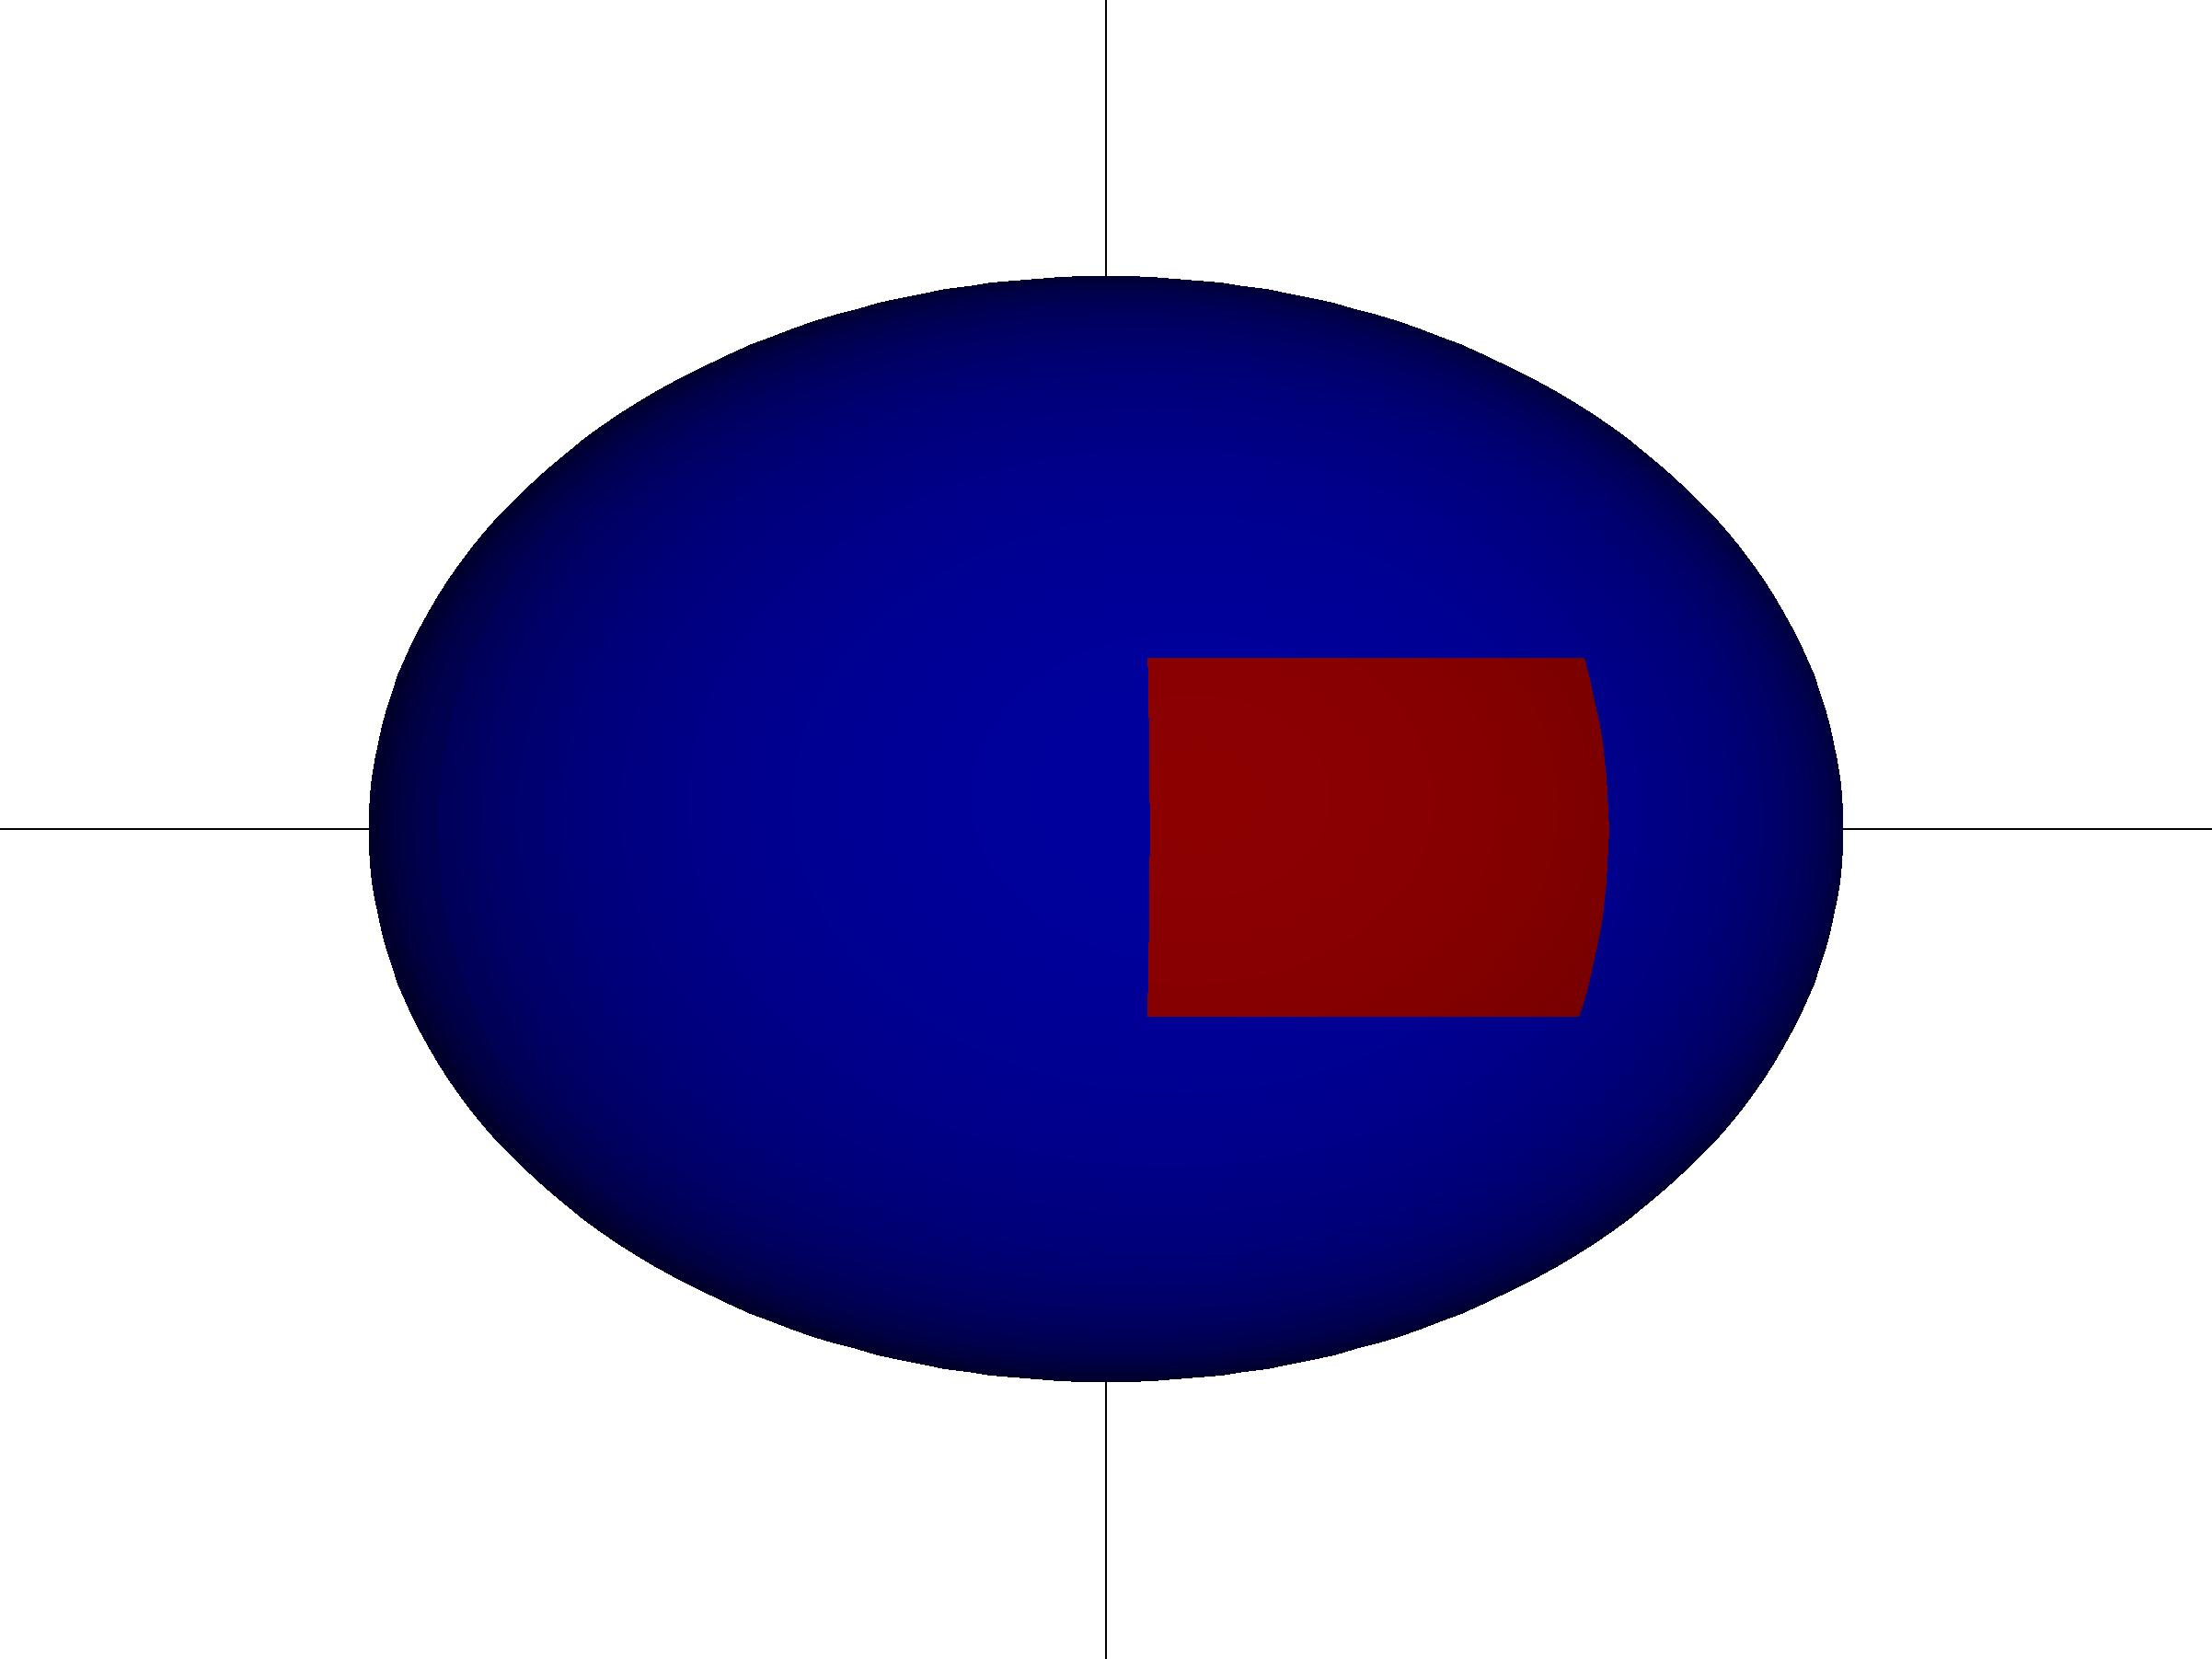
\includegraphics[width=\textwidth]{sphere2_3}
%\caption{}
%\end{subfigure}
%\begin{subfigure}{0.2\textwidth}
%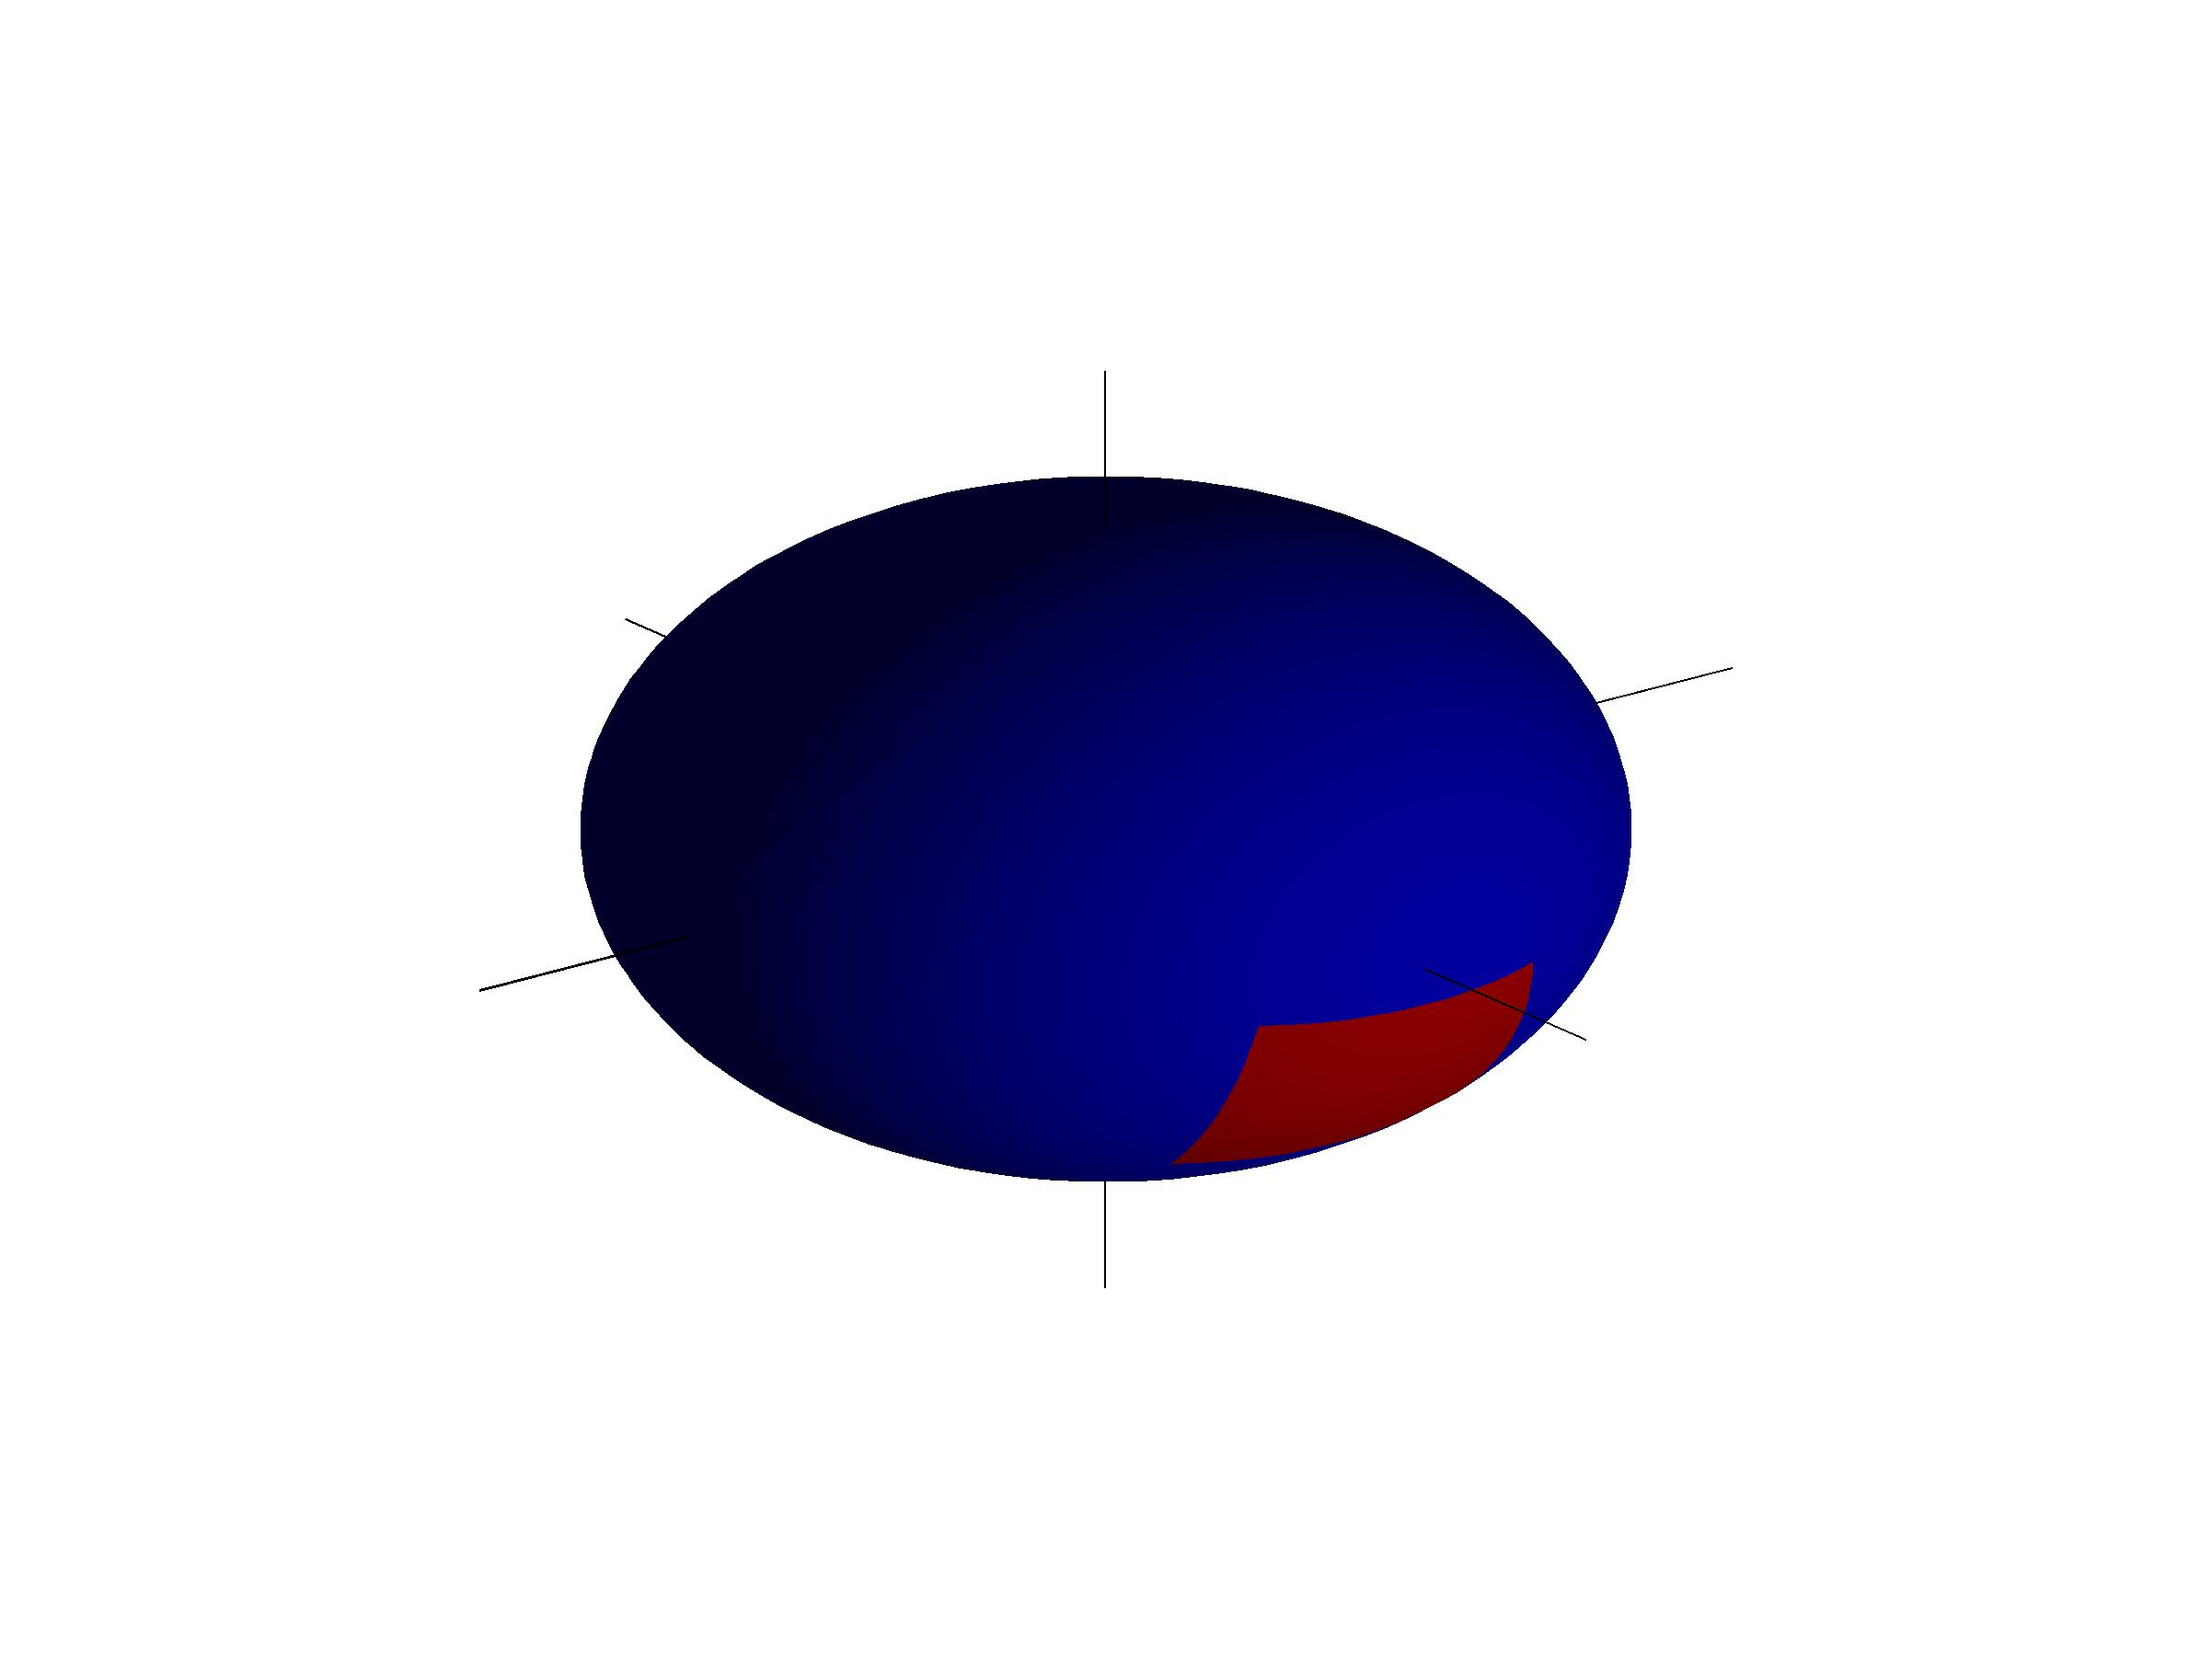
\includegraphics[width=\textwidth]{sphere_4}
%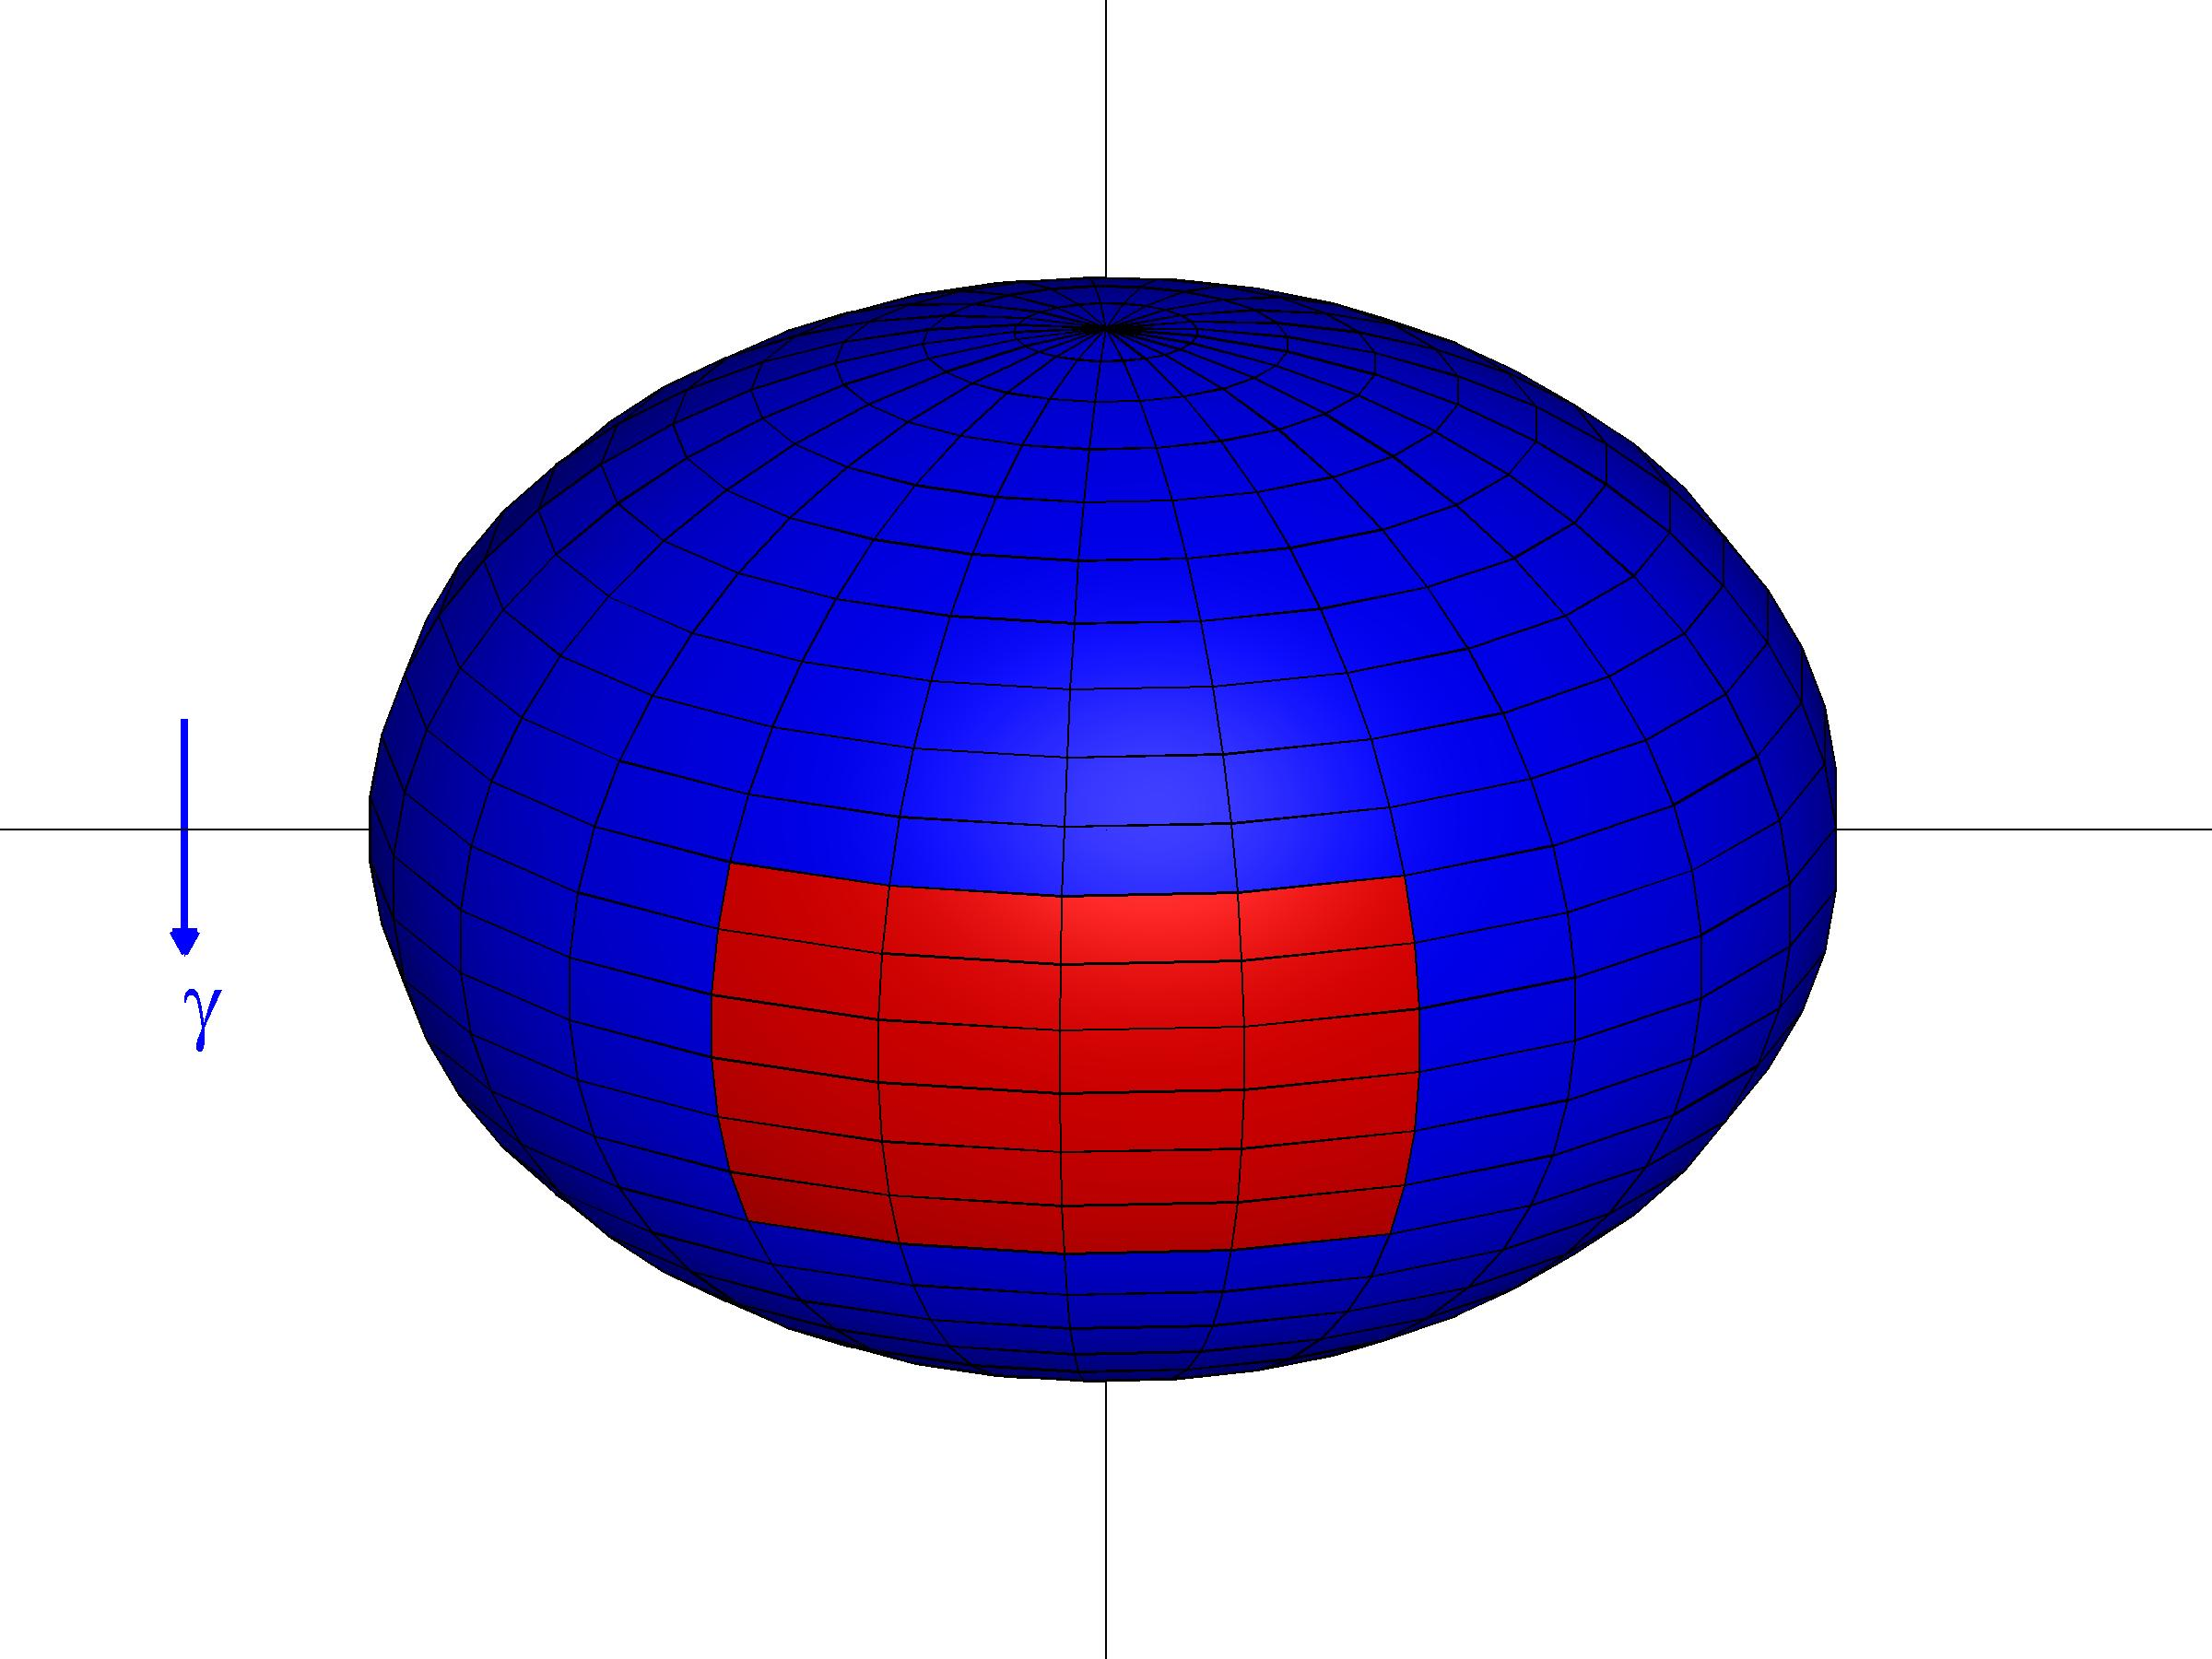
\includegraphics[width=\textwidth]{sphere2_4}
%\caption{}
%\end{subfigure}
%\caption{Illustration of how rotations in three dimensions correspond to translations and rotations in two dimensions. (a) The original image. (b) Rotation around the x-axis (Euler angle $\alpha$) in three dimensions corresponds to rotation of the image. (c) Rotation around the y-axis (Euler angle $\beta$) in three dimensions corresponds to horizontal translation. (d) Rotation around the z-axis (Euler angle $\gamma$) in three dimensions corresponds to vertical translation. The top row shows the three-dimensional spheres, and the bottom row shows the (two-dimensional) surface of the sphere in which we are interested.}
%\label{fig:SO3_picture}
%\end{figure*}

\end{document}

